%
% Result
%

% !TEX root = ../../main.tex

\chapter{Resultate\label{chap:Resulate}}

\section{Erster Versuch, parameterierbare Steuerung ohne Feedback}

  \subsection{Konfiguration}
      % !TEX root = ../main.tex

\begin{tabular}{ | l | l | }

  \hline
  \multicolumn{2}{|c|}{Simulationsparameter} \\
  \hline
  Populationsgrösse & 120 \\ \hline
  Selektionsstrategie & Turnierseletkion \\ \hline
  Iterationen & ca. 3100 \\ \hline
  Iterationsdauer & 30s \\ \hline
  Schwierigkeit erhöhen pro & 100 Generationen \\ \hline
  Steigungszunahme & 0.02 \\ \hline
  Maximale Steigung & 1.0 \\ \hline
  Höchste Y-Koordinate Zuwachs & 0.05 \\ \hline
  Wahrscheinlichkeit Mutation pro Attribut & 0.1 \\ \hline
  Ziel & Allgemeine Lösung \\ \hline

\end{tabular}


  \subsection{Auswertung}
    Es ist ein klarer aufwärts Trend zu erkennen bis etwa zur 1000. Generation (siehe Abbildung \ref{fig:graph}).
    Danach ist ein Abfall der Fitness bei den Individueen zu beobachten.
    Die Vermutung dabei ist, das der Parcour zu schwierig ist und die Individueen
    mit der grossen Steigung nicht mehr zurecht kommen. Es wird vermutet das die Implementation,
    des Feedbacksystem der Steuerung helfen wird. Ausserdem muss für die nächste Simulation
    die Parameter des Parcours anderst konfiguriert werden.
    Der Zuwachs der Steigung sollte auf 0.01 limitiert werden und der Zuwachs des höchsten Punktes
    sollte auf 0.02 gestellt werden.
      \begin{figure}
        % !TEX root = ../main.tex

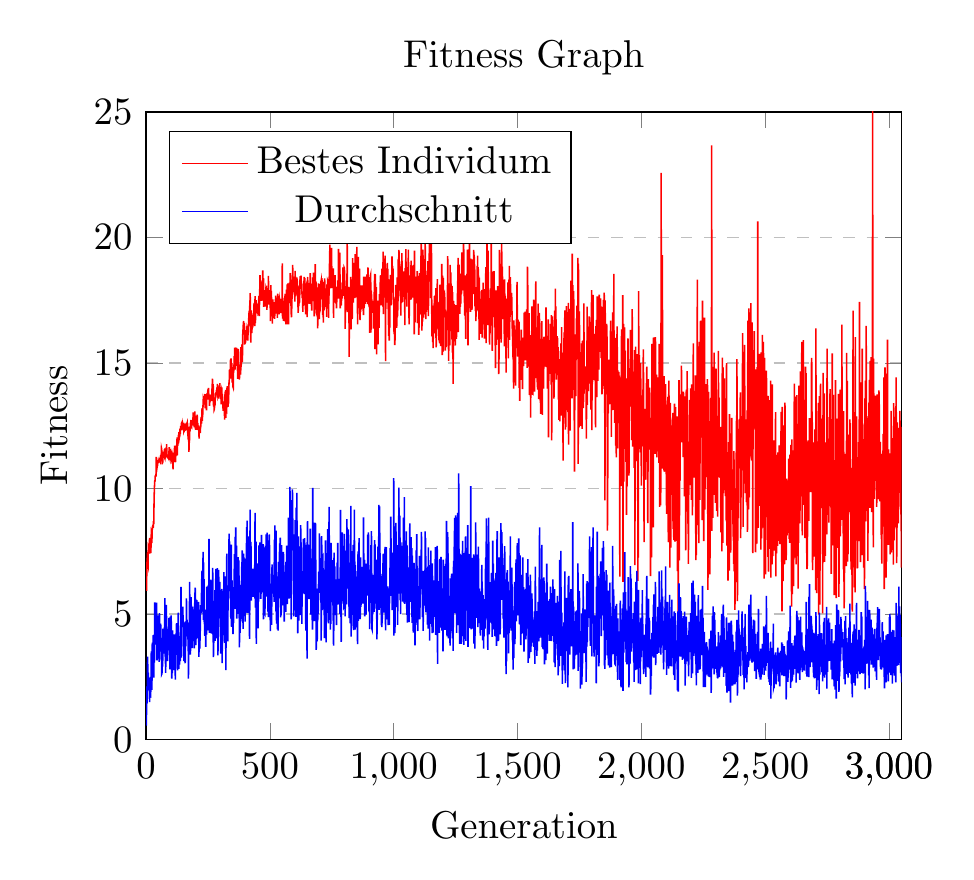
\begin{tikzpicture}[scale=1.4]
\begin{axis}[
    title={Fitness Graph},
    xlabel={Generation},
    ylabel={Fitness},
    xmin=0, xmax=3051,
    ymin=0, ymax=25,
    xtick={0,500,1000,1500,2000,2500,3000,3000},
    ytick={0,5,10,15,20,25},
    legend pos=north west,
    ymajorgrids=true,
    grid style=dashed,
]

\addplot[
    color=red,
    mark=none,
    ]
    coordinates {
	(1,6.896610736846924)(2,5.920971393585205)(3,7.004243850708008)(4,6.99455451965332)(5,7.3171892166137695)(6,7.4652557373046875)(7,6.9916205406188965)(8,6.942554950714111)(9,7.697178840637207)(10,7.666684150695801)(11,7.624490737915039)(12,7.701292991638184)(13,7.600270748138428)(14,8.032538414001465)(15,7.411534309387207)(16,7.6220831871032715)(17,7.500499248504639)(18,7.47577428817749)(19,7.471611022949219)(20,7.721786975860596)(21,8.215011596679688)(22,8.169353485107422)(23,7.824366569519043)(24,8.06535816192627)(25,8.449116706848145)(26,8.479876518249512)(27,8.449116706848145)(28,8.449116706848145)(29,8.457788467407227)(30,8.703351974487305)(31,8.585183143615723)(32,9.3861722946167)(33,9.839818954467773)(34,10.120302200317383)(35,10.303604125976562)(36,10.303604125976562)(37,10.497323036193848)(38,10.497323036193848)(39,10.506497383117676)(40,10.506497383117676)(41,11.256094932556152)(42,11.201187133789062)(43,10.883369445800781)(44,10.833419799804688)(45,10.909629821777344)(46,10.909629821777344)(47,11.00192642211914)(48,11.09583854675293)(49,11.107725143432617)(50,11.095904350280762)(51,11.111742973327637)(52,11.152694702148438)(53,11.114531517028809)(54,11.144309043884277)(55,11.121844291687012)(56,11.104765892028809)(57,11.077836990356445)(58,11.192065238952637)(59,11.298819541931152)(60,11.298819541931152)(61,11.300459861755371)(62,11.612456321716309)(63,11.568941116333008)(64,11.253467559814453)(65,10.961396217346191)(66,11.474258422851562)(67,10.999357223510742)(68,11.26171875)(69,11.34914779663086)(70,11.34914779663086)(71,11.384727478027344)(72,11.34914779663086)(73,11.312761306762695)(74,11.543015480041504)(75,11.55550765991211)(76,11.438035011291504)(77,11.432819366455078)(78,11.307319641113281)(79,11.371990203857422)(80,11.286388397216797)(81,11.404956817626953)(82,11.376131057739258)(83,11.766386032104492)(84,11.266363143920898)(85,11.261539459228516)(86,11.297901153564453)(87,11.261539459228516)(88,11.276586532592773)(89,11.235750198364258)(90,11.214592933654785)(91,11.330151557922363)(92,11.330151557922363)(93,11.616456985473633)(94,11.616456985473633)(95,11.252920150756836)(96,11.208078384399414)(97,11.580755233764648)(98,11.466822624206543)(99,11.394134521484375)(100,11.407119750976562)(101,11.307132720947266)(102,11.414825439453125)(103,11.238789558410645)(104,11.289107322692871)(105,11.38935661315918)(106,11.336462020874023)(107,11.163209915161133)(108,10.91955280303955)(109,10.762274742126465)(110,11.257829666137695)(111,11.430008888244629)(112,11.048759460449219)(113,11.365422248840332)(114,11.223052024841309)(115,11.705148696899414)(116,11.075207710266113)(117,11.433369636535645)(118,11.132770538330078)(119,11.048959732055664)(120,11.409476280212402)(121,11.437257766723633)(122,11.677118301391602)(123,11.713847160339355)(124,11.313216209411621)(125,12.03461742401123)(126,11.32917594909668)(127,11.84760856628418)(128,12.032670021057129)(129,11.96340274810791)(130,12.026735305786133)(131,12.140947341918945)(132,12.024784088134766)(133,12.253138542175293)(134,12.02083683013916)(135,12.082547187805176)(136,12.092849731445312)(137,12.37576961517334)(138,12.171459197998047)(139,12.392931938171387)(140,12.3761568069458)(141,12.435342788696289)(142,12.329865455627441)(143,12.61343002319336)(144,12.512628555297852)(145,12.504156112670898)(146,12.578330993652344)(147,12.499834060668945)(148,12.548742294311523)(149,12.486567497253418)(150,12.523869514465332)(151,12.539960861206055)(152,12.350568771362305)(153,12.402961730957031)(154,12.374781608581543)(155,12.522968292236328)(156,12.53686237335205)(157,12.44105339050293)(158,12.444380760192871)(159,12.438610076904297)(160,12.339167594909668)(161,12.34634017944336)(162,12.399177551269531)(163,12.587322235107422)(164,12.404755592346191)(165,12.59926700592041)(166,12.629351615905762)(167,12.36449146270752)(168,12.245685577392578)(169,12.317340850830078)(170,12.172144889831543)(171,11.941390991210938)(172,12.100804328918457)(173,11.457478523254395)(174,11.87552261352539)(175,11.815727233886719)(176,12.385649681091309)(177,12.371699333190918)(178,12.281112670898438)(179,12.625754356384277)(180,12.388882637023926)(181,12.734683990478516)(182,12.600780487060547)(183,12.546744346618652)(184,12.514751434326172)(185,12.716766357421875)(186,12.52918815612793)(187,12.721278190612793)(188,12.636432647705078)(189,12.605942726135254)(190,13.036943435668945)(191,12.725257873535156)(192,12.683598518371582)(193,12.775470733642578)(194,12.636879920959473)(195,12.58877182006836)(196,12.860732078552246)(197,13.071979522705078)(198,12.65569019317627)(199,12.775884628295898)(200,12.341327667236328)(201,12.574323654174805)(202,12.345996856689453)(203,12.70788288116455)(204,12.336990356445312)(205,12.800787925720215)(206,12.94461727142334)(207,12.849725723266602)(208,12.332534790039062)(209,12.43237018585205)(210,12.462204933166504)(211,12.355692863464355)(212,12.505073547363281)(213,12.302610397338867)(214,11.989819526672363)(215,12.419754981994629)(216,12.26402473449707)(217,12.27830982208252)(218,12.461591720581055)(219,12.206664085388184)(220,12.527235984802246)(221,12.465319633483887)(222,12.851350784301758)(223,12.724289894104004)(224,12.586858749389648)(225,12.836726188659668)(226,13.201416015625)(227,12.69383716583252)(228,12.919742584228516)(229,12.956737518310547)(230,13.36106014251709)(231,13.574910163879395)(232,13.529726028442383)(233,13.677021026611328)(234,13.369956016540527)(235,13.610025405883789)(236,13.646110534667969)(237,13.621960639953613)(238,13.76419448852539)(239,13.198230743408203)(240,13.398150444030762)(241,13.468585014343262)(242,13.46025276184082)(243,13.556068420410156)(244,13.116072654724121)(245,13.639655113220215)(246,13.789071083068848)(247,13.631317138671875)(248,13.549938201904297)(249,13.866223335266113)(250,13.947535514831543)(251,13.537681579589844)(252,14.010560989379883)(253,13.720366477966309)(254,13.726856231689453)(255,13.59577465057373)(256,13.290711402893066)(257,13.42927360534668)(258,13.46855640411377)(259,13.727261543273926)(260,13.607427597045898)(261,13.719259262084961)(262,13.59127426147461)(263,13.752632141113281)(264,13.584237098693848)(265,13.4862642288208)(266,13.93929672241211)(267,14.099616050720215)(268,14.37436294555664)(269,13.952011108398438)(270,13.920929908752441)(271,14.155735969543457)(272,13.353930473327637)(273,13.270903587341309)(274,13.519608497619629)(275,13.146492004394531)(276,13.177186965942383)(277,13.530131340026855)(278,13.290781021118164)(279,13.54223346710205)(280,13.785640716552734)(281,13.598223686218262)(282,13.831284523010254)(283,13.712541580200195)(284,13.930742263793945)(285,13.808953285217285)(286,14.029476165771484)(287,13.86436939239502)(288,14.167061805725098)(289,13.802409172058105)(290,13.682378768920898)(291,13.728797912597656)(292,13.741934776306152)(293,13.818764686584473)(294,13.58059024810791)(295,13.845687866210938)(296,14.116399765014648)(297,13.851978302001953)(298,14.193979263305664)(299,13.707416534423828)(300,13.862805366516113)(301,13.804529190063477)(302,13.85363483428955)(303,13.355101585388184)(304,13.988205909729004)(305,13.441354751586914)(306,14.029687881469727)(307,13.417594909667969)(308,13.771148681640625)(309,13.523871421813965)(310,13.398866653442383)(311,13.0973539352417)(312,13.468505859375)(313,13.386479377746582)(314,13.300848960876465)(315,13.401856422424316)(316,13.28846549987793)(317,12.74088191986084)(318,13.440458297729492)(319,13.856993675231934)(320,13.408331871032715)(321,13.927584648132324)(322,12.819881439208984)(323,13.362794876098633)(324,13.08174991607666)(325,13.06583023071289)(326,13.682670593261719)(327,14.070266723632812)(328,13.407576560974121)(329,14.081904411315918)(330,13.275577545166016)(331,13.280535697937012)(332,13.445354461669922)(333,13.385129928588867)(334,13.894847869873047)(335,14.2554349899292)(336,14.336638450622559)(337,14.749629974365234)(338,14.533491134643555)(339,14.737133026123047)(340,14.375664710998535)(341,15.142931938171387)(342,14.494425773620605)(343,15.186427116394043)(344,14.722400665283203)(345,14.953256607055664)(346,14.957246780395508)(347,14.509247779846191)(348,14.218650817871094)(349,14.659244537353516)(350,14.273990631103516)(351,14.048357009887695)(352,14.017618179321289)(353,14.696419715881348)(354,14.824070930480957)(355,14.804171562194824)(356,15.275089263916016)(357,15.004461288452148)(358,15.607741355895996)(359,14.739222526550293)(360,14.940775871276855)(361,15.577216148376465)(362,15.031641006469727)(363,15.494942665100098)(364,15.582799911499023)(365,15.578255653381348)(366,15.573516845703125)(367,14.882121086120605)(368,15.273076057434082)(369,14.786772727966309)(370,14.370428085327148)(371,14.952892303466797)(372,15.562775611877441)(373,15.501867294311523)(374,14.723614692687988)(375,14.88569450378418)(376,14.816357612609863)(377,14.341215133666992)(378,14.894963264465332)(379,14.887372970581055)(380,14.893570899963379)(381,14.607542991638184)(382,14.542049407958984)(383,15.635055541992188)(384,14.846089363098145)(385,15.284255981445312)(386,15.46042537689209)(387,15.742693901062012)(388,15.035285949707031)(389,15.09117603302002)(390,16.097410202026367)(391,16.234968185424805)(392,16.45393943786621)(393,16.598459243774414)(394,16.670637130737305)(395,16.411758422851562)(396,16.533767700195312)(397,16.54152488708496)(398,15.733420372009277)(399,15.9253511428833)(400,15.903125762939453)(401,16.310699462890625)(402,15.906274795532227)(403,16.110349655151367)(404,16.034774780273438)(405,16.113800048828125)(406,16.46207618713379)(407,16.047557830810547)(408,16.326208114624023)(409,16.270137786865234)(410,15.960972785949707)(411,15.891218185424805)(412,16.398386001586914)(413,16.224775314331055)(414,16.719215393066406)(415,16.84038734436035)(416,17.069629669189453)(417,16.704856872558594)(418,17.281938552856445)(419,16.804697036743164)(420,17.78761100769043)(421,17.47571563720703)(422,16.112764358520508)(423,15.815683364868164)(424,16.618494033813477)(425,17.09554672241211)(426,16.401687622070312)(427,16.19609832763672)(428,16.450380325317383)(429,16.829246520996094)(430,16.40900230407715)(431,16.47278594970703)(432,16.622474670410156)(433,16.970945358276367)(434,16.7656192779541)(435,17.01274299621582)(436,17.39260482788086)(437,16.907045364379883)(438,16.693565368652344)(439,16.470355987548828)(440,17.66329574584961)(441,16.589895248413086)(442,16.762840270996094)(443,17.439239501953125)(444,17.50002670288086)(445,17.041582107543945)(446,17.233854293823242)(447,16.980287551879883)(448,17.251365661621094)(449,17.21235466003418)(450,16.973806381225586)(451,17.157991409301758)(452,16.964820861816406)(453,16.980836868286133)(454,17.398950576782227)(455,17.55830955505371)(456,17.67156219482422)(457,16.86882209777832)(458,17.393253326416016)(459,17.90831756591797)(460,18.50388526916504)(461,18.028963088989258)(462,17.93739128112793)(463,18.117740631103516)(464,17.96273422241211)(465,17.476716995239258)(466,18.2412052154541)(467,17.83285903930664)(468,17.779539108276367)(469,18.287078857421875)(470,17.866811752319336)(471,18.6887264251709)(472,18.061986923217773)(473,18.135995864868164)(474,18.381959915161133)(475,17.237293243408203)(476,17.51453971862793)(477,17.90707778930664)(478,17.45317268371582)(479,17.31186866760254)(480,17.528715133666992)(481,17.5794734954834)(482,17.242326736450195)(483,17.621488571166992)(484,17.931734085083008)(485,17.88146209716797)(486,18.082923889160156)(487,17.341779708862305)(488,17.120285034179688)(489,17.694215774536133)(490,17.64691734313965)(491,17.56205177307129)(492,17.539939880371094)(493,17.570154190063477)(494,18.467941284179688)(495,17.5114688873291)(496,17.32908821105957)(497,17.587783813476562)(498,17.4312801361084)(499,17.90013885498047)(500,17.6003475189209)(501,17.667015075683594)(502,16.664981842041016)(503,17.55928611755371)(504,18.100555419921875)(505,17.100337982177734)(506,17.876325607299805)(507,17.091970443725586)(508,17.07583999633789)(509,17.229759216308594)(510,16.568748474121094)(511,17.336429595947266)(512,17.533706665039062)(513,16.79352378845215)(514,17.04062271118164)(515,17.240440368652344)(516,16.88433074951172)(517,17.42618751525879)(518,17.267396926879883)(519,16.758119583129883)(520,17.026018142700195)(521,17.082704544067383)(522,17.250120162963867)(523,17.681657791137695)(524,17.519264221191406)(525,17.58656120300293)(526,17.23577117919922)(527,16.972881317138672)(528,17.066720962524414)(529,17.54878044128418)(530,16.801347732543945)(531,17.7655029296875)(532,17.57737159729004)(533,17.1651611328125)(534,17.18079376220703)(535,17.54806137084961)(536,17.162410736083984)(537,16.934133529663086)(538,17.332870483398438)(539,17.547773361206055)(540,17.48558807373047)(541,17.32706069946289)(542,17.551042556762695)(543,17.334455490112305)(544,16.98756217956543)(545,17.55402183532715)(546,17.029035568237305)(547,17.4414119720459)(548,17.50503158569336)(549,17.194244384765625)(550,18.970197677612305)(551,16.764379501342773)(552,16.88475799560547)(553,17.073753356933594)(554,17.20667839050293)(555,16.680530548095703)(556,17.33775520324707)(557,16.808732986450195)(558,17.470218658447266)(559,17.586833953857422)(560,16.65488624572754)(561,17.66830825805664)(562,17.755443572998047)(563,17.534069061279297)(564,17.24616813659668)(565,16.540409088134766)(566,17.0947208404541)(567,17.918405532836914)(568,17.741464614868164)(569,16.536766052246094)(570,18.132997512817383)(571,18.002426147460938)(572,17.539030075073242)(573,18.17306900024414)(574,17.46969985961914)(575,16.53662872314453)(576,17.95696449279785)(577,17.655977249145508)(578,17.569843292236328)(579,18.197189331054688)(580,17.9415225982666)(581,17.387781143188477)(582,18.58061981201172)(583,18.525590896606445)(584,17.977840423583984)(585,17.378986358642578)(586,16.990503311157227)(587,16.81953239440918)(588,17.030508041381836)(589,18.324241638183594)(590,17.560335159301758)(591,17.88384437561035)(592,18.905712127685547)(593,18.126867294311523)(594,18.076374053955078)(595,17.9354305267334)(596,17.99142837524414)(597,18.329381942749023)(598,18.441532135009766)(599,18.169748306274414)(600,18.117191314697266)(601,17.443124771118164)(602,18.67343521118164)(603,17.784366607666016)(604,17.660329818725586)(605,18.111665725708008)(606,18.18148422241211)(607,17.896520614624023)(608,17.72356605529785)(609,18.409727096557617)(610,18.203746795654297)(611,18.269939422607422)(612,17.590715408325195)(613,17.48745346069336)(614,17.002046585083008)(615,17.17974853515625)(616,17.801300048828125)(617,17.262149810791016)(618,17.562225341796875)(619,18.092586517333984)(620,17.410348892211914)(621,18.132577896118164)(622,18.428831100463867)(623,18.43535041809082)(624,18.138437271118164)(625,17.95780372619629)(626,18.483476638793945)(627,17.990575790405273)(628,18.15911293029785)(629,18.120359420776367)(630,17.58327865600586)(631,17.76063346862793)(632,17.611360549926758)(633,17.032358169555664)(634,17.4830322265625)(635,17.442142486572266)(636,17.482545852661133)(637,17.74289894104004)(638,18.42851448059082)(639,17.295385360717773)(640,17.740453720092773)(641,18.39300537109375)(642,17.301836013793945)(643,18.117666244506836)(644,16.937496185302734)(645,17.809600830078125)(646,17.65488052368164)(647,17.49299430847168)(648,18.132434844970703)(649,18.1749324798584)(650,16.831127166748047)(651,17.154293060302734)(652,18.422574996948242)(653,18.23552703857422)(654,17.808746337890625)(655,17.5219783782959)(656,17.613082885742188)(657,18.137916564941406)(658,18.1464786529541)(659,17.35247039794922)(660,17.797698974609375)(661,17.95461082458496)(662,17.935632705688477)(663,18.57634735107422)(664,17.729406356811523)(665,17.59747314453125)(666,17.931522369384766)(667,17.388179779052734)(668,17.403108596801758)(669,17.091081619262695)(670,18.006649017333984)(671,18.16149139404297)(672,17.915058135986328)(673,18.409259796142578)(674,17.46232032775879)(675,17.778139114379883)(676,18.600627899169922)(677,17.879838943481445)(678,17.758201599121094)(679,16.859790802001953)(680,17.59970474243164)(681,17.709148406982422)(682,18.040708541870117)(683,18.941438674926758)(684,17.960865020751953)(685,17.288171768188477)(686,18.249643325805664)(687,17.168781280517578)(688,17.00166893005371)(689,16.963029861450195)(690,18.009565353393555)(691,17.72330093383789)(692,17.215044021606445)(693,16.383378982543945)(694,17.389345169067383)(695,17.646657943725586)(696,18.168046951293945)(697,17.083765029907227)(698,17.846824645996094)(699,16.992128372192383)(700,16.743921279907227)(701,18.14590835571289)(702,18.013288497924805)(703,17.05754280090332)(704,17.89238739013672)(705,17.63730812072754)(706,18.236736297607422)(707,18.288759231567383)(708,17.535554885864258)(709,18.18150520324707)(710,18.383378982543945)(711,18.12407112121582)(712,18.23920440673828)(713,16.920654296875)(714,17.840560913085938)(715,17.040498733520508)(716,16.606201171875)(717,18.235227584838867)(718,17.409217834472656)(719,17.09459114074707)(720,17.590137481689453)(721,18.365514755249023)(722,18.170103073120117)(723,17.48783302307129)(724,17.968400955200195)(725,17.581945419311523)(726,17.319746017456055)(727,17.33322525024414)(728,17.733016967773438)(729,16.836292266845703)(730,18.134410858154297)(731,17.825735092163086)(732,17.727558135986328)(733,18.295747756958008)(734,18.271501541137695)(735,17.95366668701172)(736,18.101415634155273)(737,16.794212341308594)(738,17.864255905151367)(739,17.68484878540039)(740,18.703947067260742)(741,18.662473678588867)(742,19.712881088256836)(743,18.738208770751953)(744,18.372426986694336)(745,17.97462272644043)(746,18.722919464111328)(747,18.488609313964844)(748,17.990510940551758)(749,19.587980270385742)(750,18.455381393432617)(751,18.412118911743164)(752,18.45170021057129)(753,17.982345581054688)(754,18.10601806640625)(755,18.21941375732422)(756,18.77083396911621)(757,16.793079376220703)(758,17.678194046020508)(759,17.94451141357422)(760,17.94462013244629)(761,17.51963996887207)(762,18.215917587280273)(763,18.501708984375)(764,17.409393310546875)(765,18.041275024414062)(766,17.402427673339844)(767,17.40300178527832)(768,18.034801483154297)(769,17.180646896362305)(770,17.472354888916016)(771,17.89219093322754)(772,17.629072189331055)(773,17.962848663330078)(774,18.289621353149414)(775,17.59450340270996)(776,17.595548629760742)(777,19.54677391052246)(778,17.917957305908203)(779,18.42707633972168)(780,17.899904251098633)(781,17.848243713378906)(782,19.3923282623291)(783,18.49345588684082)(784,17.174659729003906)(785,18.201662063598633)(786,17.633298873901367)(787,17.847612380981445)(788,17.291534423828125)(789,17.563005447387695)(790,17.551395416259766)(791,17.931568145751953)(792,17.573984146118164)(793,17.679527282714844)(794,18.02524185180664)(795,18.807971954345703)(796,18.266742706298828)(797,18.55715560913086)(798,18.368915557861328)(799,17.671178817749023)(800,18.79518699645996)(801,18.771150588989258)(802,18.168224334716797)(803,18.18299102783203)(804,16.355195999145508)(805,17.82869529724121)(806,17.545089721679688)(807,17.569705963134766)(808,17.643461227416992)(809,17.10116958618164)(810,18.059425354003906)(811,17.139270782470703)(812,20.46389389038086)(813,17.031076431274414)(814,17.907917022705078)(815,17.293588638305664)(816,17.407772064208984)(817,17.705738067626953)(818,18.02889633178711)(819,17.941389083862305)(820,15.248538970947266)(821,17.577363967895508)(822,18.01647186279297)(823,17.63013458251953)(824,17.28062629699707)(825,17.33887481689453)(826,18.42903709411621)(827,17.886754989624023)(828,16.3444881439209)(829,18.193639755249023)(830,17.95839500427246)(831,18.074758529663086)(832,16.74699592590332)(833,16.83186149597168)(834,19.1778621673584)(835,17.68035125732422)(836,18.192890167236328)(837,17.404254913330078)(838,18.434127807617188)(839,18.05166244506836)(840,18.01498031616211)(841,18.988664627075195)(842,18.1341609954834)(843,17.588441848754883)(844,19.337432861328125)(845,18.807310104370117)(846,17.90471076965332)(847,18.770063400268555)(848,18.232820510864258)(849,17.611492156982422)(850,18.708051681518555)(851,19.62554359436035)(852,18.051090240478516)(853,19.093399047851562)(854,16.536596298217773)(855,17.17746925354004)(856,18.042551040649414)(857,19.2263126373291)(858,18.53277587890625)(859,17.45316505432129)(860,18.381675720214844)(861,17.635957717895508)(862,18.761863708496094)(863,17.043010711669922)(864,16.708148956298828)(865,17.79802894592285)(866,17.027441024780273)(867,17.531877517700195)(868,17.297645568847656)(869,17.949684143066406)(870,18.089649200439453)(871,17.956335067749023)(872,18.09125328063965)(873,17.261884689331055)(874,17.2825870513916)(875,17.17685317993164)(876,17.769380569458008)(877,17.08500862121582)(878,16.904075622558594)(879,18.44379234313965)(880,17.190635681152344)(881,17.267887115478516)(882,17.48872184753418)(883,18.01375389099121)(884,17.359384536743164)(885,18.372793197631836)(886,18.093381881713867)(887,18.43771743774414)(888,17.496763229370117)(889,18.128990173339844)(890,18.437538146972656)(891,17.432998657226562)(892,18.525869369506836)(893,18.400480270385742)(894,17.341812133789062)(895,18.158021926879883)(896,18.806550979614258)(897,17.77849769592285)(898,17.781837463378906)(899,18.271997451782227)(900,17.32317352294922)(901,17.231224060058594)(902,18.422931671142578)(903,16.200305938720703)(904,17.823631286621094)(905,16.532888412475586)(906,18.481830596923828)(907,18.523481369018555)(908,16.205984115600586)(909,17.04328155517578)(910,17.882055282592773)(911,16.9930362701416)(912,17.53521156311035)(913,17.179031372070312)(914,17.302928924560547)(915,17.072622299194336)(916,17.409780502319336)(917,17.473718643188477)(918,16.37294578552246)(919,16.958431243896484)(920,16.6685791015625)(921,17.646343231201172)(922,18.027774810791016)(923,18.54929542541504)(924,15.554770469665527)(925,18.53348159790039)(926,18.475568771362305)(927,17.475635528564453)(928,16.897985458374023)(929,17.35509490966797)(930,18.025772094726562)(931,15.343116760253906)(932,16.56534194946289)(933,15.901972770690918)(934,17.30405044555664)(935,17.486164093017578)(936,17.119014739990234)(937,15.743388175964355)(938,17.291872024536133)(939,17.269058227539062)(940,16.62289810180664)(941,16.39790153503418)(942,17.738866806030273)(943,17.60429573059082)(944,17.41463279724121)(945,17.77133560180664)(946,18.40511703491211)(947,18.49362564086914)(948,17.909427642822266)(949,17.292476654052734)(950,17.792102813720703)(951,17.65395164489746)(952,18.756345748901367)(953,18.55228614807129)(954,18.646411895751953)(955,17.961618423461914)(956,17.24530601501465)(957,19.441234588623047)(958,16.943635940551758)(959,18.441810607910156)(960,18.592763900756836)(961,17.60573387145996)(962,18.57741355895996)(963,18.991025924682617)(964,18.320228576660156)(965,19.272762298583984)(966,18.545957565307617)(967,15.073798179626465)(968,18.00469207763672)(969,18.314682006835938)(970,17.81855583190918)(971,18.51441192626953)(972,18.339569091796875)(973,17.406574249267578)(974,18.983823776245117)(975,18.21582794189453)(976,18.753713607788086)(977,18.232463836669922)(978,17.153121948242188)(979,16.527158737182617)(980,16.08197593688965)(981,18.328285217285156)(982,15.892411231994629)(983,17.776752471923828)(984,16.40996742248535)(985,17.511945724487305)(986,18.248170852661133)(987,18.509443283081055)(988,17.58552360534668)(989,17.325061798095703)(990,17.324260711669922)(991,17.839345932006836)(992,18.030668258666992)(993,19.25086784362793)(994,18.657909393310547)(995,18.86896514892578)(996,17.887805938720703)(997,18.75856590270996)(998,18.10013198852539)(999,17.52740478515625)(1000,17.64490509033203)(1001,16.283782958984375)(1002,16.152599334716797)(1003,17.17962074279785)(1004,15.71060562133789)(1005,15.803339958190918)(1006,17.217649459838867)(1007,16.5941104888916)(1008,17.33932113647461)(1009,18.108659744262695)(1010,17.5216064453125)(1011,16.57155990600586)(1012,16.398221969604492)(1013,16.94219207763672)(1014,18.415193557739258)(1015,16.8189754486084)(1016,17.198564529418945)(1017,17.097333908081055)(1018,19.12967872619629)(1019,17.67856788635254)(1020,19.008819580078125)(1021,19.502330780029297)(1022,19.252050399780273)(1023,17.881746292114258)(1024,18.84555435180664)(1025,18.114606857299805)(1026,18.624515533447266)(1027,17.847763061523438)(1028,17.370243072509766)(1029,16.891515731811523)(1030,18.54139518737793)(1031,19.04388999938965)(1032,18.031248092651367)(1033,19.37653160095215)(1034,18.464008331298828)(1035,17.456220626831055)(1036,17.465003967285156)(1037,18.0467529296875)(1038,17.637630462646484)(1039,18.64369773864746)(1040,18.559738159179688)(1041,18.631643295288086)(1042,18.299453735351562)(1043,18.056272506713867)(1044,17.922000885009766)(1045,16.507558822631836)(1046,18.783283233642578)(1047,18.211118698120117)(1048,18.23401641845703)(1049,19.53792381286621)(1050,18.50743293762207)(1051,18.812265396118164)(1052,18.72528076171875)(1053,17.241966247558594)(1054,18.31548309326172)(1055,18.305816650390625)(1056,17.88450813293457)(1057,18.717052459716797)(1058,18.038320541381836)(1059,19.517629623413086)(1060,18.66360092163086)(1061,17.789634704589844)(1062,16.538036346435547)(1063,17.07171058654785)(1064,18.485788345336914)(1065,17.514101028442383)(1066,18.03562355041504)(1067,17.917861938476562)(1068,18.182300567626953)(1069,17.524803161621094)(1070,19.080976486206055)(1071,17.532243728637695)(1072,18.196292877197266)(1073,18.37624740600586)(1074,17.982221603393555)(1075,18.762866973876953)(1076,18.87238311767578)(1077,17.66657829284668)(1078,17.605785369873047)(1079,18.233657836914062)(1080,18.906160354614258)(1081,17.731618881225586)(1082,18.332860946655273)(1083,16.136098861694336)(1084,19.47319221496582)(1085,17.165964126586914)(1086,16.620220184326172)(1087,17.905689239501953)(1088,18.443859100341797)(1089,18.080610275268555)(1090,17.37164306640625)(1091,18.09977149963379)(1092,17.804689407348633)(1093,17.88966178894043)(1094,18.044954299926758)(1095,18.656259536743164)(1096,16.58856201171875)(1097,16.835176467895508)(1098,17.423770904541016)(1099,17.123634338378906)(1100,18.466466903686523)(1101,16.121627807617188)(1102,16.409873962402344)(1103,18.243860244750977)(1104,16.897968292236328)(1105,18.581275939941406)(1106,16.924497604370117)(1107,18.255826950073242)(1108,17.741304397583008)(1109,18.608137130737305)(1110,19.083858489990234)(1111,19.775789260864258)(1112,19.021791458129883)(1113,17.334177017211914)(1114,16.294607162475586)(1115,18.008039474487305)(1116,17.380306243896484)(1117,16.64554786682129)(1118,19.51567268371582)(1119,17.865337371826172)(1120,17.34895896911621)(1121,16.804271697998047)(1122,19.136363983154297)(1123,18.74629020690918)(1124,18.59928321838379)(1125,18.24888038635254)(1126,17.876785278320312)(1127,20.442014694213867)(1128,16.93694496154785)(1129,18.683897018432617)(1130,16.749723434448242)(1131,18.503393173217773)(1132,17.03281593322754)(1133,17.342634201049805)(1134,17.694053649902344)(1135,17.46282196044922)(1136,18.31092643737793)(1137,18.217763900756836)(1138,19.05657386779785)(1139,17.662734985351562)(1140,16.870182037353516)(1141,18.02027130126953)(1142,18.637407302856445)(1143,18.51588249206543)(1144,19.97096061706543)(1145,18.590848922729492)(1146,20.71241569519043)(1147,18.401029586791992)(1148,19.574846267700195)(1149,17.585153579711914)(1150,18.056020736694336)(1151,19.221477508544922)(1152,19.835044860839844)(1153,18.848459243774414)(1154,16.06218147277832)(1155,16.535987854003906)(1156,17.11984634399414)(1157,15.830833435058594)(1158,17.219114303588867)(1159,15.592066764831543)(1160,16.280195236206055)(1161,17.28277015686035)(1162,16.479461669921875)(1163,16.411836624145508)(1164,17.659847259521484)(1165,16.488983154296875)(1166,16.180984497070312)(1167,17.69753074645996)(1168,16.568845748901367)(1169,16.44268226623535)(1170,17.983020782470703)(1171,15.623106956481934)(1172,15.721076011657715)(1173,16.648691177368164)(1174,16.86603546142578)(1175,16.780832290649414)(1176,18.340116500854492)(1177,16.577177047729492)(1178,17.117969512939453)(1179,17.409395217895508)(1180,17.11310577392578)(1181,16.320261001586914)(1182,16.062776565551758)(1183,15.904569625854492)(1184,17.43531608581543)(1185,15.780439376831055)(1186,15.972946166992188)(1187,18.124094009399414)(1188,17.23781394958496)(1189,17.697540283203125)(1190,15.667722702026367)(1191,17.817493438720703)(1192,17.149503707885742)(1193,17.119428634643555)(1194,18.94780731201172)(1195,17.16680908203125)(1196,15.311445236206055)(1197,18.480905532836914)(1198,17.46550941467285)(1199,15.458311080932617)(1200,18.390480041503906)(1201,17.653919219970703)(1202,17.268741607666016)(1203,17.33856773376465)(1204,17.757308959960938)(1205,17.78297233581543)(1206,17.62115478515625)(1207,17.114370346069336)(1208,15.49565601348877)(1209,16.298208236694336)(1210,15.71839714050293)(1211,15.861797332763672)(1212,15.630369186401367)(1213,17.053871154785156)(1214,16.652244567871094)(1215,16.31068229675293)(1216,16.910747528076172)(1217,17.656023025512695)(1218,19.258617401123047)(1219,18.005924224853516)(1220,17.847427368164062)(1221,15.757488250732422)(1222,15.084696769714355)(1223,18.16999626159668)(1224,16.054672241210938)(1225,17.58127784729004)(1226,17.324426651000977)(1227,15.704453468322754)(1228,18.90821647644043)(1229,16.81869888305664)(1230,17.81656265258789)(1231,18.61109733581543)(1232,16.498868942260742)(1233,16.81498908996582)(1234,17.57107925415039)(1235,15.944726943969727)(1236,18.072994232177734)(1237,15.410137176513672)(1238,17.818819046020508)(1239,16.1085205078125)(1240,14.1694917678833)(1241,17.37095069885254)(1242,17.471193313598633)(1243,16.749692916870117)(1244,17.34499740600586)(1245,16.358949661254883)(1246,17.214204788208008)(1247,16.525829315185547)(1248,16.095624923706055)(1249,15.697778701782227)(1250,16.952341079711914)(1251,17.30976104736328)(1252,16.46176528930664)(1253,15.959982872009277)(1254,16.150611877441406)(1255,16.59105682373047)(1256,16.8662109375)(1257,16.853553771972656)(1258,18.236841201782227)(1259,18.303346633911133)(1260,19.185352325439453)(1261,16.22780990600586)(1262,18.669822692871094)(1263,17.822742462158203)(1264,18.921253204345703)(1265,18.269620895385742)(1266,17.22494888305664)(1267,16.953380584716797)(1268,18.313045501708984)(1269,17.232494354248047)(1270,17.83070182800293)(1271,17.3701171875)(1272,18.554759979248047)(1273,17.739219665527344)(1274,17.803857803344727)(1275,19.406600952148438)(1276,18.761817932128906)(1277,18.145668029785156)(1278,17.89775848388672)(1279,18.367027282714844)(1280,18.375755310058594)(1281,19.326316833496094)(1282,19.986648559570312)(1283,19.338228225708008)(1284,17.966928482055664)(1285,17.639896392822266)(1286,17.393024444580078)(1287,16.885929107666016)(1288,18.487571716308594)(1289,18.21127700805664)(1290,16.698535919189453)(1291,15.957511901855469)(1292,18.36859130859375)(1293,17.874879837036133)(1294,17.40974235534668)(1295,18.28990936279297)(1296,18.54629898071289)(1297,17.01820945739746)(1298,19.51806640625)(1299,19.443456649780273)(1300,15.705748558044434)(1301,16.75603485107422)(1302,19.167736053466797)(1303,19.05282211303711)(1304,18.91093635559082)(1305,19.176414489746094)(1306,19.904369354248047)(1307,18.642486572265625)(1308,17.189964294433594)(1309,18.135629653930664)(1310,17.03540802001953)(1311,19.160648345947266)(1312,17.912412643432617)(1313,17.601064682006836)(1314,18.2322940826416)(1315,17.485008239746094)(1316,17.121341705322266)(1317,19.1318359375)(1318,18.627819061279297)(1319,18.830703735351562)(1320,18.699722290039062)(1321,17.745973587036133)(1322,18.547588348388672)(1323,19.509572982788086)(1324,18.702878952026367)(1325,19.30658531188965)(1326,18.604957580566406)(1327,18.930387496948242)(1328,17.26604652404785)(1329,17.352508544921875)(1330,17.066781997680664)(1331,17.308656692504883)(1332,16.665498733520508)(1333,17.739299774169922)(1334,17.043777465820312)(1335,18.025348663330078)(1336,17.06598472595215)(1337,18.869962692260742)(1338,17.859704971313477)(1339,19.278013229370117)(1340,17.11441421508789)(1341,18.81356430053711)(1342,18.567697525024414)(1343,18.246549606323242)(1344,17.530681610107422)(1345,15.923298835754395)(1346,18.39605140686035)(1347,16.681108474731445)(1348,16.594697952270508)(1349,17.310468673706055)(1350,16.1574649810791)(1351,16.378894805908203)(1352,17.455141067504883)(1353,16.455909729003906)(1354,17.251100540161133)(1355,17.76387596130371)(1356,17.91168975830078)(1357,16.007465362548828)(1358,17.286468505859375)(1359,16.902441024780273)(1360,17.169464111328125)(1361,18.19655418395996)(1362,17.094615936279297)(1363,17.053918838500977)(1364,17.939674377441406)(1365,17.116785049438477)(1366,15.974668502807617)(1367,17.772510528564453)(1368,17.575389862060547)(1369,17.117521286010742)(1370,17.37629508972168)(1371,17.823205947875977)(1372,18.82231903076172)(1373,15.794529914855957)(1374,17.246543884277344)(1375,17.096113204956055)(1376,19.181236267089844)(1377,20.27115821838379)(1378,18.572542190551758)(1379,16.81955337524414)(1380,16.507333755493164)(1381,19.4724178314209)(1382,18.157655715942383)(1383,17.870248794555664)(1384,17.431257247924805)(1385,16.873252868652344)(1386,16.670127868652344)(1387,15.734734535217285)(1388,16.317068099975586)(1389,16.203916549682617)(1390,16.605205535888672)(1391,16.957942962646484)(1392,17.976531982421875)(1393,16.85081672668457)(1394,20.48255157470703)(1395,17.208984375)(1396,18.196456909179688)(1397,16.50918197631836)(1398,15.4869966506958)(1399,18.64400863647461)(1400,18.37197494506836)(1401,17.737085342407227)(1402,17.881322860717773)(1403,16.82566261291504)(1404,18.275882720947266)(1405,18.662336349487305)(1406,17.864994049072266)(1407,17.431598663330078)(1408,16.422454833984375)(1409,17.694477081298828)(1410,15.815741539001465)(1411,14.796163558959961)(1412,16.818828582763672)(1413,17.89337921142578)(1414,15.72538948059082)(1415,16.246055603027344)(1416,15.929676055908203)(1417,16.97348403930664)(1418,17.06047821044922)(1419,17.192705154418945)(1420,18.066259384155273)(1421,17.17508888244629)(1422,17.48954963684082)(1423,16.949573516845703)(1424,14.561742782592773)(1425,15.075654029846191)(1426,16.284381866455078)(1427,19.501686096191406)(1428,18.079008102416992)(1429,18.7606258392334)(1430,15.964054107666016)(1431,18.945858001708984)(1432,18.30729103088379)(1433,18.63629722595215)(1434,15.811838150024414)(1435,16.809221267700195)(1436,19.853086471557617)(1437,17.270198822021484)(1438,17.29966163635254)(1439,18.83534049987793)(1440,16.745214462280273)(1441,16.99994468688965)(1442,18.190059661865234)(1443,16.951242446899414)(1444,17.78291893005371)(1445,18.31499671936035)(1446,16.590871810913086)(1447,15.65995979309082)(1448,18.335336685180664)(1449,16.275531768798828)(1450,17.676496505737305)(1451,17.361433029174805)(1452,16.286619186401367)(1453,15.825398445129395)(1454,14.613356590270996)(1455,17.556907653808594)(1456,16.267778396606445)(1457,17.034894943237305)(1458,16.43804168701172)(1459,16.232114791870117)(1460,16.90883445739746)(1461,18.21073341369629)(1462,17.34109115600586)(1463,15.184423446655273)(1464,17.979402542114258)(1465,18.31913948059082)(1466,16.75747299194336)(1467,18.873680114746094)(1468,15.91658878326416)(1469,17.452890396118164)(1470,16.83481788635254)(1471,18.423559188842773)(1472,17.862529754638672)(1473,17.209686279296875)(1474,16.96710968017578)(1475,17.03078842163086)(1476,17.795927047729492)(1477,17.48017692565918)(1478,16.742202758789062)(1479,16.253477096557617)(1480,15.999582290649414)(1481,15.564518928527832)(1482,15.147003173828125)(1483,15.32008171081543)(1484,13.980080604553223)(1485,16.7008113861084)(1486,16.38112449645996)(1487,15.195009231567383)(1488,15.49087905883789)(1489,15.328588485717773)(1490,14.925463676452637)(1491,15.301995277404785)(1492,14.10077953338623)(1493,16.241533279418945)(1494,16.335166931152344)(1495,16.50080108642578)(1496,16.75613784790039)(1497,15.861920356750488)(1498,18.232927322387695)(1499,17.03151512145996)(1500,15.808440208435059)(1501,15.25087833404541)(1502,16.728893280029297)(1503,16.106462478637695)(1504,15.839588165283203)(1505,15.561720848083496)(1506,16.650131225585938)(1507,14.01351547241211)(1508,15.89306640625)(1509,13.48766040802002)(1510,15.462831497192383)(1511,15.714695930480957)(1512,14.334249496459961)(1513,14.492754936218262)(1514,15.400757789611816)(1515,16.327056884765625)(1516,15.856392860412598)(1517,15.397785186767578)(1518,14.507230758666992)(1519,15.341203689575195)(1520,13.962470054626465)(1521,15.101656913757324)(1522,16.008726119995117)(1523,15.379005432128906)(1524,14.880403518676758)(1525,15.12635612487793)(1526,15.164862632751465)(1527,17.010421752929688)(1528,15.616095542907715)(1529,16.333829879760742)(1530,15.917522430419922)(1531,17.04840850830078)(1532,15.104162216186523)(1533,15.950316429138184)(1534,16.13345718383789)(1535,15.181187629699707)(1536,16.423965454101562)(1537,17.1401309967041)(1538,15.863286018371582)(1539,14.802478790283203)(1540,18.835371017456055)(1541,18.64145278930664)(1542,15.252758026123047)(1543,14.860902786254883)(1544,15.976715087890625)(1545,16.94204330444336)(1546,15.833353996276855)(1547,16.988306045532227)(1548,13.727374076843262)(1549,15.4297513961792)(1550,15.11625862121582)(1551,16.113513946533203)(1552,14.401131629943848)(1553,12.82667064666748)(1554,15.677597999572754)(1555,15.210691452026367)(1556,15.65297794342041)(1557,14.211874961853027)(1558,17.253026962280273)(1559,14.781416893005371)(1560,16.180845260620117)(1561,13.761462211608887)(1562,13.75529670715332)(1563,17.04637336730957)(1564,16.576101303100586)(1565,17.518938064575195)(1566,17.446731567382812)(1567,14.810110092163086)(1568,16.98430061340332)(1569,13.8577299118042)(1570,15.766066551208496)(1571,16.55983543395996)(1572,15.44575023651123)(1573,17.974361419677734)(1574,18.25533676147461)(1575,14.399514198303223)(1576,16.320995330810547)(1577,15.577948570251465)(1578,14.804969787597656)(1579,14.239361763000488)(1580,14.320306777954102)(1581,13.935927391052246)(1582,15.405702590942383)(1583,17.362003326416016)(1584,15.317452430725098)(1585,13.559205055236816)(1586,16.172073364257812)(1587,15.248995780944824)(1588,16.99468421936035)(1589,16.606977462768555)(1590,14.335453033447266)(1591,13.516355514526367)(1592,15.861201286315918)(1593,12.972865104675293)(1594,15.485054969787598)(1595,15.618886947631836)(1596,15.358638763427734)(1597,16.032800674438477)(1598,16.667476654052734)(1599,14.051575660705566)(1600,12.932698249816895)(1601,15.672415733337402)(1602,15.959142684936523)(1603,15.263527870178223)(1604,15.407583236694336)(1605,13.983331680297852)(1606,15.013144493103027)(1607,16.04802131652832)(1608,15.608404159545898)(1609,15.052087783813477)(1610,15.83161449432373)(1611,15.869022369384766)(1612,15.198169708251953)(1613,14.854353904724121)(1614,15.62369155883789)(1615,17.211400985717773)(1616,15.74549674987793)(1617,14.84032154083252)(1618,15.061203956604004)(1619,16.082366943359375)(1620,15.675628662109375)(1621,13.975878715515137)(1622,14.591682434082031)(1623,14.580146789550781)(1624,16.733354568481445)(1625,12.035429000854492)(1626,14.364643096923828)(1627,14.789082527160645)(1628,15.912562370300293)(1629,15.074233055114746)(1630,14.681528091430664)(1631,14.668607711791992)(1632,14.566630363464355)(1633,16.557762145996094)(1634,15.020561218261719)(1635,16.279356002807617)(1636,14.142388343811035)(1637,16.905752182006836)(1638,11.918410301208496)(1639,15.797256469726562)(1640,15.872124671936035)(1641,16.853702545166016)(1642,15.543771743774414)(1643,14.24233627319336)(1644,16.20958709716797)(1645,16.447877883911133)(1646,14.602547645568848)(1647,13.586426734924316)(1648,13.96826171875)(1649,15.473028182983398)(1650,17.089763641357422)(1651,16.198396682739258)(1652,15.552793502807617)(1653,17.958782196044922)(1654,14.58398723602295)(1655,17.251832962036133)(1656,15.122873306274414)(1657,14.3391752243042)(1658,15.198495864868164)(1659,14.96870231628418)(1660,16.06914710998535)(1661,15.106300354003906)(1662,15.99878978729248)(1663,14.729757308959961)(1664,15.629817962646484)(1665,13.53751277923584)(1666,15.468422889709473)(1667,12.734256744384766)(1668,15.156354904174805)(1669,13.168729782104492)(1670,14.152386665344238)(1671,12.670900344848633)(1672,14.748708724975586)(1673,14.813228607177734)(1674,13.850711822509766)(1675,15.784067153930664)(1676,12.903223991394043)(1677,13.471226692199707)(1678,16.429229736328125)(1679,14.259753227233887)(1680,14.648544311523438)(1681,14.200986862182617)(1682,14.87718391418457)(1683,13.590581893920898)(1684,11.112940788269043)(1685,14.387308120727539)(1686,15.403675079345703)(1687,15.274208068847656)(1688,16.223207473754883)(1689,14.502394676208496)(1690,15.785848617553711)(1691,17.096620559692383)(1692,13.522253036499023)(1693,12.348994255065918)(1694,12.786384582519531)(1695,12.738972663879395)(1696,14.557389259338379)(1697,17.26839828491211)(1698,13.56398868560791)(1699,13.492507934570312)(1700,15.077383041381836)(1701,13.265632629394531)(1702,13.562614440917969)(1703,13.076769828796387)(1704,13.07345962524414)(1705,17.396913528442383)(1706,11.745465278625488)(1707,16.943233489990234)(1708,14.724194526672363)(1709,13.464384078979492)(1710,16.555360794067383)(1711,17.156681060791016)(1712,12.303178787231445)(1713,16.86115074157715)(1714,16.828960418701172)(1715,17.0650634765625)(1716,18.27630043029785)(1717,16.273279190063477)(1718,18.17293357849121)(1719,16.17950439453125)(1720,13.58663272857666)(1721,19.353321075439453)(1722,17.022872924804688)(1723,18.096349716186523)(1724,17.808792114257812)(1725,13.928763389587402)(1726,17.859943389892578)(1727,17.510692596435547)(1728,14.148918151855469)(1729,13.063000679016113)(1730,10.673580169677734)(1731,13.222885131835938)(1732,15.913124084472656)(1733,16.139341354370117)(1734,15.97036075592041)(1735,13.679708480834961)(1736,15.116113662719727)(1737,15.384279251098633)(1738,16.7740421295166)(1739,15.884565353393555)(1740,17.28748893737793)(1741,16.424224853515625)(1742,15.97080135345459)(1743,15.150177001953125)(1744,19.18729019165039)(1745,10.98363208770752)(1746,18.96121597290039)(1747,16.646053314208984)(1748,15.487069129943848)(1749,12.434381484985352)(1750,17.053497314453125)(1751,13.31214714050293)(1752,13.70571231842041)(1753,15.429085731506348)(1754,14.972946166992188)(1755,12.492060661315918)(1756,12.601439476013184)(1757,14.358601570129395)(1758,13.585535049438477)(1759,15.783745765686035)(1760,12.776103019714355)(1761,12.377349853515625)(1762,15.880642890930176)(1763,13.799867630004883)(1764,14.7852783203125)(1765,15.899660110473633)(1766,13.204144477844238)(1767,14.038007736206055)(1768,17.372623443603516)(1769,13.783380508422852)(1770,14.296184539794922)(1771,13.950775146484375)(1772,14.530111312866211)(1773,14.864837646484375)(1774,14.601523399353027)(1775,14.59156608581543)(1776,14.192497253417969)(1777,13.902613639831543)(1778,11.990684509277344)(1779,13.879977226257324)(1780,13.55456829071045)(1781,17.246320724487305)(1782,13.334460258483887)(1783,14.777503967285156)(1784,14.347466468811035)(1785,16.44718360900879)(1786,13.87827205657959)(1787,15.237237930297852)(1788,14.525243759155273)(1789,16.85361099243164)(1790,14.177241325378418)(1791,16.637348175048828)(1792,15.865472793579102)(1793,15.34805965423584)(1794,15.41280746459961)(1795,14.44144058227539)(1796,13.145256996154785)(1797,16.816499710083008)(1798,15.417481422424316)(1799,17.899169921875)(1800,12.325292587280273)(1801,14.225688934326172)(1802,14.217422485351562)(1803,14.785877227783203)(1804,15.621744155883789)(1805,17.71253204345703)(1806,14.327007293701172)(1807,15.720187187194824)(1808,16.1618595123291)(1809,14.881410598754883)(1810,15.851725578308105)(1811,14.51401424407959)(1812,14.555150985717773)(1813,15.80169677734375)(1814,15.443397521972656)(1815,12.435770988464355)(1816,16.464353561401367)(1817,14.004314422607422)(1818,13.697725296020508)(1819,16.71480941772461)(1820,13.638277053833008)(1821,16.243553161621094)(1822,17.65595054626465)(1823,14.759481430053711)(1824,14.291635513305664)(1825,16.05620765686035)(1826,15.778265953063965)(1827,17.070682525634766)(1828,14.733806610107422)(1829,16.637786865234375)(1830,17.720840454101562)(1831,17.363977432250977)(1832,16.778913497924805)(1833,15.446606636047363)(1834,15.700691223144531)(1835,17.57248878479004)(1836,17.25405502319336)(1837,15.596183776855469)(1838,15.199644088745117)(1839,17.239355087280273)(1840,16.73681640625)(1841,13.75562572479248)(1842,15.602788925170898)(1843,15.582375526428223)(1844,13.970858573913574)(1845,17.22714614868164)(1846,16.209854125976562)(1847,17.511930465698242)(1848,15.329092025756836)(1849,15.11087417602539)(1850,17.80052947998047)(1851,16.784536361694336)(1852,14.596077919006348)(1853,9.52491283416748)(1854,17.492528915405273)(1855,13.748104095458984)(1856,15.027031898498535)(1857,14.634818077087402)(1858,15.625753402709961)(1859,13.816683769226074)(1860,16.562782287597656)(1861,16.23455047607422)(1862,15.333593368530273)(1863,8.326824188232422)(1864,9.263449668884277)(1865,14.30173110961914)(1866,14.80307674407959)(1867,12.995856285095215)(1868,14.332908630371094)(1869,15.135685920715332)(1870,13.520207405090332)(1871,13.729986190795898)(1872,13.754745483398438)(1873,14.70008373260498)(1874,13.363677024841309)(1875,15.846441268920898)(1876,16.683687210083008)(1877,14.394912719726562)(1878,15.294600486755371)(1879,12.055152893066406)(1880,14.871968269348145)(1881,15.478487968444824)(1882,15.885628700256348)(1883,15.068920135498047)(1884,17.01413917541504)(1885,13.456332206726074)(1886,13.133979797363281)(1887,16.95907974243164)(1888,16.03754997253418)(1889,18.546009063720703)(1890,13.746158599853516)(1891,15.006202697753906)(1892,12.617546081542969)(1893,15.225003242492676)(1894,13.145966529846191)(1895,15.39385986328125)(1896,11.704728126525879)(1897,15.99754810333252)(1898,11.899333953857422)(1899,11.238543510437012)(1900,14.983834266662598)(1901,15.03126335144043)(1902,16.455211639404297)(1903,15.061630249023438)(1904,11.5958890914917)(1905,14.707111358642578)(1906,12.860306739807129)(1907,13.578102111816406)(1908,12.604606628417969)(1909,14.645773887634277)(1910,14.191422462463379)(1911,14.498685836791992)(1912,14.393340110778809)(1913,6.495210647583008)(1914,13.213603973388672)(1915,13.097195625305176)(1916,11.640595436096191)(1917,10.300514221191406)(1918,10.253378868103027)(1919,10.101263999938965)(1920,16.33720588684082)(1921,13.513439178466797)(1922,14.55647087097168)(1923,14.999707221984863)(1924,14.792440414428711)(1925,17.703462600708008)(1926,6.286880016326904)(1927,16.069936752319336)(1928,16.55997085571289)(1929,10.279569625854492)(1930,13.5911283493042)(1931,13.509020805358887)(1932,16.420652389526367)(1933,15.107068061828613)(1934,11.575729370117188)(1935,15.493474960327148)(1936,13.830982208251953)(1937,14.014409065246582)(1938,11.062938690185547)(1939,14.123370170593262)(1940,8.950811386108398)(1941,14.391130447387695)(1942,10.084308624267578)(1943,12.991434097290039)(1944,13.706085205078125)(1945,13.662242889404297)(1946,15.98529052734375)(1947,11.174812316894531)(1948,12.894157409667969)(1949,14.028398513793945)(1950,10.51901626586914)(1951,12.643580436706543)(1952,13.550518989562988)(1953,14.795990943908691)(1954,14.445956230163574)(1955,14.66532039642334)(1956,16.321073532104492)(1957,15.558255195617676)(1958,13.25976848602295)(1959,13.862434387207031)(1960,16.214279174804688)(1961,11.932369232177734)(1962,15.82183837890625)(1963,17.146032333374023)(1964,15.301600456237793)(1965,11.668898582458496)(1966,13.210379600524902)(1967,13.659961700439453)(1968,13.489776611328125)(1969,13.663936614990234)(1970,13.719950675964355)(1971,10.8230619430542)(1972,14.799553871154785)(1973,15.508286476135254)(1974,6.953574180603027)(1975,13.321967124938965)(1976,13.949235916137695)(1977,15.657106399536133)(1978,13.169548034667969)(1979,11.087400436401367)(1980,11.950281143188477)(1981,13.791601181030273)(1982,14.721392631530762)(1983,11.920682907104492)(1984,15.356371879577637)(1985,13.901490211486816)(1986,6.321865081787109)(1987,15.146581649780273)(1988,7.243292808532715)(1989,17.862796783447266)(1990,14.51883316040039)(1991,14.420161247253418)(1992,15.312773704528809)(1993,12.58939266204834)(1994,13.019312858581543)(1995,14.335362434387207)(1996,11.436583518981934)(1997,14.99277400970459)(1998,13.752540588378906)(1999,12.877398490905762)(2000,10.113286972045898)(2001,10.833298683166504)(2002,13.70793342590332)(2003,13.614378929138184)(2004,13.050128936767578)(2005,11.681802749633789)(2006,13.675542831420898)(2007,14.014913558959961)(2008,15.545912742614746)(2009,14.014565467834473)(2010,12.43839168548584)(2011,7.867124080657959)(2012,11.840251922607422)(2013,10.343457221984863)(2014,13.16835880279541)(2015,12.989051818847656)(2016,11.856776237487793)(2017,10.356828689575195)(2018,12.21264362335205)(2019,11.061064720153809)(2020,12.908236503601074)(2021,14.315961837768555)(2022,14.855956077575684)(2023,13.667082786560059)(2024,12.951395034790039)(2025,11.582005500793457)(2026,8.619353294372559)(2027,11.273820877075195)(2028,14.353947639465332)(2029,13.353752136230469)(2030,11.554306030273438)(2031,12.065241813659668)(2032,12.852507591247559)(2033,14.016328811645508)(2034,12.509533882141113)(2035,12.7426118850708)(2036,12.001614570617676)(2037,6.516263484954834)(2038,12.81480884552002)(2039,9.660470962524414)(2040,11.018036842346191)(2041,7.256417274475098)(2042,13.556361198425293)(2043,15.765213012695312)(2044,8.45659065246582)(2045,12.490110397338867)(2046,10.440322875976562)(2047,11.449784278869629)(2048,8.4503812789917)(2049,16.008346557617188)(2050,13.443573951721191)(2051,13.4364652633667)(2052,16.025659561157227)(2053,14.738560676574707)(2054,13.638813972473145)(2055,13.241498947143555)(2056,11.38031005859375)(2057,16.034486770629883)(2058,13.037237167358398)(2059,12.657633781433105)(2060,13.900193214416504)(2061,13.573349952697754)(2062,14.541749000549316)(2063,11.245881080627441)(2064,13.250475883483887)(2065,12.681428909301758)(2066,14.431221961975098)(2067,13.669364929199219)(2068,11.633793830871582)(2069,14.412433624267578)(2070,12.801666259765625)(2071,11.021943092346191)(2072,15.763282775878906)(2073,13.618902206420898)(2074,9.266268730163574)(2075,12.744470596313477)(2076,14.897647857666016)(2077,9.989130020141602)(2078,9.33178424835205)(2079,11.25252914428711)(2080,22.575008392333984)(2081,14.574921607971191)(2082,11.246408462524414)(2083,10.795214653015137)(2084,13.06373119354248)(2085,19.293642044067383)(2086,12.68932819366455)(2087,10.796385765075684)(2088,12.473831176757812)(2089,12.454833030700684)(2090,12.741568565368652)(2091,10.722834587097168)(2092,14.475892066955566)(2093,10.701252937316895)(2094,10.704812049865723)(2095,12.742086410522461)(2096,12.848531723022461)(2097,11.089910507202148)(2098,14.160810470581055)(2099,12.710819244384766)(2100,11.679430961608887)(2101,10.041949272155762)(2102,8.991848945617676)(2103,9.731461524963379)(2104,12.852499961853027)(2105,13.34566593170166)(2106,11.181745529174805)(2107,13.652817726135254)(2108,9.44493579864502)(2109,7.8657307624816895)(2110,12.002129554748535)(2111,14.302289962768555)(2112,13.2605619430542)(2113,10.849922180175781)(2114,12.056236267089844)(2115,6.844902992248535)(2116,12.72775650024414)(2117,13.414436340332031)(2118,9.899568557739258)(2119,7.645036220550537)(2120,10.854853630065918)(2121,10.710238456726074)(2122,12.511045455932617)(2123,10.971399307250977)(2124,9.961555480957031)(2125,12.74136734008789)(2126,10.53175163269043)(2127,13.013096809387207)(2128,8.392882347106934)(2129,9.923779487609863)(2130,10.746216773986816)(2131,7.949191570281982)(2132,12.376258850097656)(2133,11.480132102966309)(2134,13.386527061462402)(2135,8.347880363464355)(2136,7.888033866882324)(2137,12.98295783996582)(2138,13.237874031066895)(2139,11.502660751342773)(2140,9.533679962158203)(2141,7.9122185707092285)(2142,11.99731731414795)(2143,10.07422161102295)(2144,11.995630264282227)(2145,12.87557315826416)(2146,6.707098484039307)(2147,12.2024507522583)(2148,8.764589309692383)(2149,4.769046306610107)(2150,10.91401195526123)(2151,9.673970222473145)(2152,14.319091796875)(2153,7.137584209442139)(2154,8.965509414672852)(2155,11.268068313598633)(2156,10.316106796264648)(2157,13.749861717224121)(2158,12.757521629333496)(2159,12.405081748962402)(2160,13.27653980255127)(2161,12.939388275146484)(2162,14.891304016113281)(2163,11.841405868530273)(2164,12.43212890625)(2165,11.879608154296875)(2166,12.636680603027344)(2167,12.279824256896973)(2168,12.598699569702148)(2169,11.249028205871582)(2170,13.860359191894531)(2171,13.376273155212402)(2172,13.5420560836792)(2173,13.264694213867188)(2174,9.688613891601562)(2175,13.673572540283203)(2176,12.18127155303955)(2177,11.802791595458984)(2178,12.81660270690918)(2179,7.540347576141357)(2180,7.669098854064941)(2181,13.797201156616211)(2182,13.933370590209961)(2183,12.43804931640625)(2184,9.480189323425293)(2185,14.680941581726074)(2186,12.25521469116211)(2187,10.727190971374512)(2188,8.60490608215332)(2189,9.484763145446777)(2190,6.997071743011475)(2191,8.719653129577637)(2192,11.787040710449219)(2193,11.473040580749512)(2194,12.185340881347656)(2195,13.516622543334961)(2196,10.988065719604492)(2197,13.526535987854004)(2198,10.137133598327637)(2199,13.986406326293945)(2200,13.178205490112305)(2201,13.860051155090332)(2202,9.549829483032227)(2203,14.145767211914062)(2204,14.055798530578613)(2205,13.057541847229004)(2206,8.926570892333984)(2207,9.658990859985352)(2208,12.8939847946167)(2209,14.259848594665527)(2210,15.777933120727539)(2211,11.54293155670166)(2212,10.435199737548828)(2213,11.507956504821777)(2214,12.879169464111328)(2215,11.861063957214355)(2216,13.887622833251953)(2217,11.336852073669434)(2218,14.506330490112305)(2219,12.565184593200684)(2220,7.151656627655029)(2221,9.324790000915527)(2222,7.352583408355713)(2223,11.792043685913086)(2224,12.656758308410645)(2225,10.421019554138184)(2226,18.318880081176758)(2227,11.606151580810547)(2228,13.716259002685547)(2229,8.543403625488281)(2230,11.483201026916504)(2231,12.187155723571777)(2232,7.8267035484313965)(2233,12.79568099975586)(2234,15.846151351928711)(2235,11.626248359680176)(2236,9.544259071350098)(2237,11.445032119750977)(2238,13.746600151062012)(2239,16.690399169921875)(2240,13.347296714782715)(2241,12.71298599243164)(2242,12.031332015991211)(2243,13.547749519348145)(2244,13.964941024780273)(2245,16.51028823852539)(2246,8.746365547180176)(2247,17.48037338256836)(2248,10.662243843078613)(2249,12.998143196105957)(2250,12.00312328338623)(2251,8.892523765563965)(2252,7.90701150894165)(2253,9.936270713806152)(2254,11.42795467376709)(2255,16.804981231689453)(2256,9.160477638244629)(2257,13.797627449035645)(2258,9.99656867980957)(2259,14.158125877380371)(2260,11.736363410949707)(2261,11.124178886413574)(2262,10.648035049438477)(2263,12.375385284423828)(2264,13.094053268432617)(2265,13.740303039550781)(2266,10.455549240112305)(2267,14.354619979858398)(2268,10.084568977355957)(2269,5.96515417098999)(2270,12.492140769958496)(2271,7.68700647354126)(2272,13.851583480834961)(2273,11.22721004486084)(2274,10.576194763183594)(2275,10.821748733520508)(2276,8.506135940551758)(2277,6.5820183753967285)(2278,10.866869926452637)(2279,10.840006828308105)(2280,12.106352806091309)(2281,13.613381385803223)(2282,10.653498649597168)(2283,12.748923301696777)(2284,23.668546676635742)(2285,8.313148498535156)(2286,13.489060401916504)(2287,14.433490753173828)(2288,14.40106201171875)(2289,8.833111763000488)(2290,13.930163383483887)(2291,14.84831428527832)(2292,11.69173812866211)(2293,12.067376136779785)(2294,15.417595863342285)(2295,13.548093795776367)(2296,9.748933792114258)(2297,12.534034729003906)(2298,12.558830261230469)(2299,9.429671287536621)(2300,11.5944185256958)(2301,12.29692268371582)(2302,14.773453712463379)(2303,9.974761962890625)(2304,9.11120319366455)(2305,10.177760124206543)(2306,9.643575668334961)(2307,12.025925636291504)(2308,8.881954193115234)(2309,12.387571334838867)(2310,10.826701164245605)(2311,15.48635482788086)(2312,12.824991226196289)(2313,11.658834457397461)(2314,13.622543334960938)(2315,11.039523124694824)(2316,10.465850830078125)(2317,10.4585599899292)(2318,12.395258903503418)(2319,11.476367950439453)(2320,12.454618453979492)(2321,8.250539779663086)(2322,10.347061157226562)(2323,11.233542442321777)(2324,11.772674560546875)(2325,7.499231338500977)(2326,11.663270950317383)(2327,15.21766185760498)(2328,12.178912162780762)(2329,7.835810661315918)(2330,14.82175350189209)(2331,9.81928825378418)(2332,11.230188369750977)(2333,14.351191520690918)(2334,12.578940391540527)(2335,14.38906478881836)(2336,10.357268333435059)(2337,10.462075233459473)(2338,13.588813781738281)(2339,9.694401741027832)(2340,11.675965309143066)(2341,10.696409225463867)(2342,11.330008506774902)(2343,8.6895112991333)(2344,14.999332427978516)(2345,10.526408195495605)(2346,7.730041027069092)(2347,8.350652694702148)(2348,8.767376899719238)(2349,10.898797035217285)(2350,6.332857608795166)(2351,8.863887786865234)(2352,9.005237579345703)(2353,11.847482681274414)(2354,10.933979034423828)(2355,6.7303996086120605)(2356,12.959893226623535)(2357,9.823643684387207)(2358,9.166728019714355)(2359,8.141281127929688)(2360,7.452330589294434)(2361,7.5498738288879395)(2362,11.451358795166016)(2363,9.850940704345703)(2364,12.062752723693848)(2365,12.810303688049316)(2366,9.151609420776367)(2367,10.760610580444336)(2368,9.91836929321289)(2369,9.950435638427734)(2370,8.697535514831543)(2371,8.203986167907715)(2372,8.252737998962402)(2373,6.994556903839111)(2374,11.492921829223633)(2375,6.6961164474487305)(2376,7.080205917358398)(2377,7.8288493156433105)(2378,5.168750286102295)(2379,7.21837043762207)(2380,10.011016845703125)(2381,6.275956630706787)(2382,6.391942977905273)(2383,10.727622985839844)(2384,12.695201873779297)(2385,11.551570892333984)(2386,15.156180381774902)(2387,11.464977264404297)(2388,5.513301849365234)(2389,6.694655418395996)(2390,12.376482009887695)(2391,10.995647430419922)(2392,8.82091999053955)(2393,11.300849914550781)(2394,11.822917938232422)(2395,12.744840621948242)(2396,12.054956436157227)(2397,12.769868850708008)(2398,10.971163749694824)(2399,13.399657249450684)(2400,13.831372261047363)(2401,8.029311180114746)(2402,9.110211372375488)(2403,10.690528869628906)(2404,11.494089126586914)(2405,10.88785171508789)(2406,12.884316444396973)(2407,12.239134788513184)(2408,13.171388626098633)(2409,16.192848205566406)(2410,14.364118576049805)(2411,8.472589492797852)(2412,11.058362007141113)(2413,12.533607482910156)(2414,10.807160377502441)(2415,11.229466438293457)(2416,13.216621398925781)(2417,15.723875045776367)(2418,12.342462539672852)(2419,11.102251052856445)(2420,9.814716339111328)(2421,10.366663932800293)(2422,12.755165100097656)(2423,12.246578216552734)(2424,9.455554962158203)(2425,12.145071029663086)(2426,10.606812477111816)(2427,13.111427307128906)(2428,8.27489948272705)(2429,8.421749114990234)(2430,16.68536949157715)(2431,11.980093002319336)(2432,12.68136215209961)(2433,9.166915893554688)(2434,17.180370330810547)(2435,14.368242263793945)(2436,9.651480674743652)(2437,15.02700138092041)(2438,11.278343200683594)(2439,12.171510696411133)(2440,12.545249938964844)(2441,13.029594421386719)(2442,17.388673782348633)(2443,15.289815902709961)(2444,12.694750785827637)(2445,11.117998123168945)(2446,13.662437438964844)(2447,16.61393165588379)(2448,11.089564323425293)(2449,12.278992652893066)(2450,7.424822807312012)(2451,12.596540451049805)(2452,12.3411865234375)(2453,15.515106201171875)(2454,15.457520484924316)(2455,12.579122543334961)(2456,16.266159057617188)(2457,14.017810821533203)(2458,13.13821792602539)(2459,13.565119743347168)(2460,12.859728813171387)(2461,7.462732315063477)(2462,7.81968879699707)(2463,14.742865562438965)(2464,9.08343505859375)(2465,12.487872123718262)(2466,7.8074188232421875)(2467,10.044478416442871)(2468,14.837455749511719)(2469,12.62069034576416)(2470,20.643550872802734)(2471,8.896526336669922)(2472,8.434738159179688)(2473,13.639920234680176)(2474,11.66171932220459)(2475,11.932655334472656)(2476,12.505449295043945)(2477,15.108501434326172)(2478,15.366218566894531)(2479,11.711862564086914)(2480,9.312503814697266)(2481,9.90137004852295)(2482,12.586819648742676)(2483,7.567458629608154)(2484,15.421100616455078)(2485,9.088729858398438)(2486,8.012923240661621)(2487,10.90458869934082)(2488,9.126514434814453)(2489,16.120685577392578)(2490,11.489423751831055)(2491,8.438958168029785)(2492,9.901758193969727)(2493,15.844745635986328)(2494,13.646055221557617)(2495,15.154487609863281)(2496,6.40918493270874)(2497,11.57955551147461)(2498,15.202740669250488)(2499,10.887935638427734)(2500,11.44953727722168)(2501,9.529698371887207)(2502,6.583811283111572)(2503,14.447867393493652)(2504,11.841985702514648)(2505,14.69727611541748)(2506,13.763367652893066)(2507,12.460525512695312)(2508,9.706024169921875)(2509,11.756416320800781)(2510,8.834927558898926)(2511,7.280852317810059)(2512,13.692249298095703)(2513,6.748526573181152)(2514,6.690079689025879)(2515,13.518765449523926)(2516,7.600207805633545)(2517,12.943269729614258)(2518,12.97193717956543)(2519,11.00578784942627)(2520,9.977286338806152)(2521,10.587008476257324)(2522,14.293827056884766)(2523,6.455185890197754)(2524,10.992321968078613)(2525,11.101164817810059)(2526,9.754576683044434)(2527,9.623536109924316)(2528,6.975029945373535)(2529,14.149808883666992)(2530,8.923784255981445)(2531,7.30978536605835)(2532,8.694247245788574)(2533,8.510981559753418)(2534,11.917961120605469)(2535,10.166766166687012)(2536,7.5313720703125)(2537,8.825019836425781)(2538,9.540946006774902)(2539,8.781084060668945)(2540,7.833899974822998)(2541,11.083943367004395)(2542,13.038939476013184)(2543,6.49999475479126)(2544,8.729049682617188)(2545,8.193572998046875)(2546,7.4166975021362305)(2547,11.34048080444336)(2548,10.029536247253418)(2549,8.150710105895996)(2550,7.718278884887695)(2551,11.442587852478027)(2552,9.303646087646484)(2553,7.949731826782227)(2554,10.750582695007324)(2555,8.476115226745605)(2556,7.9182448387146)(2557,11.719463348388672)(2558,10.161977767944336)(2559,8.345154762268066)(2560,7.7848219871521)(2561,10.198637962341309)(2562,8.826216697692871)(2563,11.71039867401123)(2564,12.22021484375)(2565,13.057914733886719)(2566,11.355276107788086)(2567,7.311516284942627)(2568,5.106220722198486)(2569,13.253615379333496)(2570,10.709094047546387)(2571,8.145710945129395)(2572,6.308127403259277)(2573,9.75290298461914)(2574,12.515753746032715)(2575,10.36129379272461)(2576,7.287919044494629)(2577,9.57622241973877)(2578,6.980566501617432)(2579,8.684078216552734)(2580,13.418736457824707)(2581,9.301641464233398)(2582,10.388760566711426)(2583,7.979373931884766)(2584,9.296807289123535)(2585,7.146395683288574)(2586,9.697515487670898)(2587,10.394196510314941)(2588,9.05061149597168)(2589,8.131412506103516)(2590,8.997264862060547)(2591,10.324630737304688)(2592,9.131980895996094)(2593,8.455612182617188)(2594,8.393646240234375)(2595,11.19446849822998)(2596,10.021439552307129)(2597,7.998130798339844)(2598,10.33004379272461)(2599,7.831487655639648)(2600,11.348725318908691)(2601,10.766035079956055)(2602,8.98300838470459)(2603,9.885063171386719)(2604,11.737975120544434)(2605,10.1852388381958)(2606,6.458330154418945)(2607,5.295248508453369)(2608,11.959470748901367)(2609,9.011053085327148)(2610,5.791354656219482)(2611,9.153633117675781)(2612,7.832010746002197)(2613,11.51529312133789)(2614,10.963569641113281)(2615,6.114931106567383)(2616,9.028225898742676)(2617,12.450815200805664)(2618,14.174417495727539)(2619,7.550021648406982)(2620,13.313496589660645)(2621,8.522940635681152)(2622,11.986255645751953)(2623,7.251677513122559)(2624,13.65832805633545)(2625,6.979292392730713)(2626,11.900866508483887)(2627,9.004508972167969)(2628,13.715851783752441)(2629,10.253802299499512)(2630,8.883967399597168)(2631,11.963770866394043)(2632,10.787034034729004)(2633,6.0131611824035645)(2634,11.406988143920898)(2635,7.83650016784668)(2636,14.099154472351074)(2637,10.36572551727295)(2638,13.416626930236816)(2639,10.173787117004395)(2640,8.613030433654785)(2641,9.457514762878418)(2642,14.671514511108398)(2643,11.441569328308105)(2644,9.964957237243652)(2645,9.683667182922363)(2646,12.267560005187988)(2647,12.529382705688477)(2648,15.837114334106445)(2649,9.70507526397705)(2650,8.136821746826172)(2651,9.992571830749512)(2652,13.765954971313477)(2653,9.34634780883789)(2654,15.913527488708496)(2655,10.298954010009766)(2656,10.378510475158691)(2657,12.735393524169922)(2658,11.713176727294922)(2659,13.277859687805176)(2660,10.817248344421387)(2661,8.024101257324219)(2662,13.518890380859375)(2663,14.85757827758789)(2664,8.911797523498535)(2665,14.599684715270996)(2666,11.368317604064941)(2667,11.425724029541016)(2668,7.471508979797363)(2669,6.792577266693115)(2670,6.93233585357666)(2671,8.22936725616455)(2672,10.452652931213379)(2673,9.144645690917969)(2674,11.91588020324707)(2675,9.405678749084473)(2676,8.715556144714355)(2677,10.590686798095703)(2678,10.125649452209473)(2679,12.80884838104248)(2680,10.64792537689209)(2681,11.434953689575195)(2682,10.16741943359375)(2683,10.887749671936035)(2684,9.85334587097168)(2685,11.484889030456543)(2686,10.060491561889648)(2687,14.967018127441406)(2688,15.207645416259766)(2689,12.104572296142578)(2690,13.064748764038086)(2691,7.183115482330322)(2692,6.754398345947266)(2693,11.066119194030762)(2694,11.84246826171875)(2695,8.770833969116211)(2696,8.517885208129883)(2697,8.807693481445312)(2698,7.291373252868652)(2699,10.811283111572266)(2700,7.824018478393555)(2701,12.351499557495117)(2702,7.942290306091309)(2703,8.932571411132812)(2704,5.953444004058838)(2705,16.383127212524414)(2706,7.797211170196533)(2707,9.955445289611816)(2708,5.836019515991211)(2709,8.270708084106445)(2710,8.657561302185059)(2711,9.002389907836914)(2712,11.87720775604248)(2713,8.363003730773926)(2714,12.752470970153809)(2715,13.412961959838867)(2716,4.977917194366455)(2717,9.877422332763672)(2718,6.659541130065918)(2719,13.682287216186523)(2720,8.521953582763672)(2721,5.373564720153809)(2722,9.02094554901123)(2723,14.022150993347168)(2724,14.17464542388916)(2725,9.220075607299805)(2726,12.781206130981445)(2727,9.378485679626465)(2728,12.183366775512695)(2729,10.044116973876953)(2730,12.095130920410156)(2731,12.124168395996094)(2732,5.027795791625977)(2733,9.219938278198242)(2734,14.610689163208008)(2735,11.928669929504395)(2736,12.360776901245117)(2737,8.799357414245605)(2738,8.205286026000977)(2739,13.791291236877441)(2740,7.077659606933594)(2741,7.980143070220947)(2742,10.436139106750488)(2743,7.31962251663208)(2744,11.843096733093262)(2745,10.272314071655273)(2746,10.5399169921875)(2747,8.871088027954102)(2748,9.92534351348877)(2749,8.17796516418457)(2750,15.57525634765625)(2751,13.548036575317383)(2752,11.65992259979248)(2753,12.84714412689209)(2754,11.212573051452637)(2755,10.800457000732422)(2756,11.985771179199219)(2757,8.646041870117188)(2758,11.22685432434082)(2759,9.784500122070312)(2760,11.75794792175293)(2761,9.892674446105957)(2762,13.961109161376953)(2763,9.988777160644531)(2764,12.762298583984375)(2765,9.247446060180664)(2766,11.762779235839844)(2767,6.605226039886475)(2768,8.69326400756836)(2769,9.832565307617188)(2770,10.93691635131836)(2771,15.385475158691406)(2772,7.7385029792785645)(2773,10.949954986572266)(2774,9.397002220153809)(2775,13.730866432189941)(2776,8.736737251281738)(2777,9.155920028686523)(2778,11.135910987854004)(2779,5.7515950202941895)(2780,10.375152587890625)(2781,8.724181175231934)(2782,9.552751541137695)(2783,6.919101715087891)(2784,14.320368766784668)(2785,12.393660545349121)(2786,9.768205642700195)(2787,5.636532306671143)(2788,12.283286094665527)(2789,12.786709785461426)(2790,10.917572021484375)(2791,8.565692901611328)(2792,9.771130561828613)(2793,8.811454772949219)(2794,7.639275074005127)(2795,9.77407169342041)(2796,13.770602226257324)(2797,12.485329627990723)(2798,5.686692714691162)(2799,10.848235130310059)(2800,9.763962745666504)(2801,10.65619945526123)(2802,12.520233154296875)(2803,13.93771743774414)(2804,8.091014862060547)(2805,10.7527494430542)(2806,12.90507984161377)(2807,9.025089263916016)(2808,13.677152633666992)(2809,12.343256950378418)(2810,16.53101348876953)(2811,8.755273818969727)(2812,10.818028450012207)(2813,9.52855110168457)(2814,9.439401626586914)(2815,9.467265129089355)(2816,6.775440692901611)(2817,13.082313537597656)(2818,7.3338518142700195)(2819,5.2242021560668945)(2820,6.013862609863281)(2821,8.014067649841309)(2822,9.185565948486328)(2823,7.816834926605225)(2824,10.690028190612793)(2825,11.380215644836426)(2826,7.198842525482178)(2827,10.825242042541504)(2828,6.908046722412109)(2829,15.400701522827148)(2830,12.184102058410645)(2831,8.605737686157227)(2832,14.287935256958008)(2833,7.093271732330322)(2834,9.70933723449707)(2835,7.384689807891846)(2836,10.866579055786133)(2837,11.620595932006836)(2838,9.745462417602539)(2839,12.143290519714355)(2840,11.20947551727295)(2841,9.05746841430664)(2842,12.7560396194458)(2843,11.869988441467285)(2844,12.601142883300781)(2845,9.954365730285645)(2846,7.81964111328125)(2847,6.8695387840271)(2848,6.88538932800293)(2849,9.58947467803955)(2850,10.818263053894043)(2851,5.489498615264893)(2852,5.097744464874268)(2853,8.011061668395996)(2854,7.468523979187012)(2855,17.08629035949707)(2856,7.440361022949219)(2857,6.982118606567383)(2858,10.988462448120117)(2859,13.043853759765625)(2860,6.063562393188477)(2861,10.135882377624512)(2862,9.967551231384277)(2863,5.862209320068359)(2864,16.026742935180664)(2865,7.927083492279053)(2866,8.144142150878906)(2867,11.092734336853027)(2868,9.567584037780762)(2869,12.87012004852295)(2870,9.807158470153809)(2871,11.248242378234863)(2872,6.85017728805542)(2873,6.8542609214782715)(2874,8.845294952392578)(2875,10.915159225463867)(2876,8.340407371520996)(2877,9.685806274414062)(2878,11.847844123840332)(2879,7.90928316116333)(2880,12.358426094055176)(2881,17.43281364440918)(2882,12.854955673217773)(2883,13.169523239135742)(2884,14.230987548828125)(2885,7.067490100860596)(2886,13.30368709564209)(2887,11.024856567382812)(2888,13.855045318603516)(2889,9.472058296203613)(2890,13.418835639953613)(2891,7.7372026443481445)(2892,15.574445724487305)(2893,7.3450236320495605)(2894,12.591136932373047)(2895,8.573025703430176)(2896,11.358078956604004)(2897,11.522024154663086)(2898,6.852118015289307)(2899,8.837566375732422)(2900,9.622726440429688)(2901,5.998038291931152)(2902,11.301122665405273)(2903,13.592386245727539)(2904,10.666337966918945)(2905,14.299224853515625)(2906,8.835103034973145)(2907,8.694010734558105)(2908,16.480310440063477)(2909,11.076401710510254)(2910,9.960285186767578)(2911,12.881692886352539)(2912,12.50722599029541)(2913,12.646839141845703)(2914,10.461095809936523)(2915,7.1161699295043945)(2916,12.306066513061523)(2917,11.744750022888184)(2918,10.631190299987793)(2919,13.422447204589844)(2920,9.92326545715332)(2921,14.323369026184082)(2922,11.848414421081543)(2923,9.232354164123535)(2924,15.083097457885742)(2925,11.061383247375488)(2926,12.052752494812012)(2927,11.235250473022461)(2928,15.233875274658203)(2929,9.650694847106934)(2930,9.057828903198242)(2931,10.029756546020508)(2932,11.795689582824707)(2933,9.242839813232422)(2934,27.62238311767578)(2935,10.604371070861816)(2936,8.919875144958496)(2937,7.660231113433838)(2938,15.177000999450684)(2939,11.968920707702637)(2940,12.580801010131836)(2941,9.58757209777832)(2942,12.879681587219238)(2943,10.8132963180542)(2944,12.130399703979492)(2945,13.703182220458984)(2946,10.813112258911133)(2947,10.301437377929688)(2948,11.574334144592285)(2949,11.813486099243164)(2950,9.266060829162598)(2951,9.564032554626465)(2952,13.747634887695312)(2953,10.765559196472168)(2954,10.600622177124023)(2955,11.850102424621582)(2956,10.65810489654541)(2957,11.252137184143066)(2958,9.578944206237793)(2959,13.90932559967041)(2960,13.81856918334961)(2961,13.08787727355957)(2962,9.832318305969238)(2963,9.48766040802002)(2964,11.388443946838379)(2965,11.859431266784668)(2966,11.22757625579834)(2967,10.756824493408203)(2968,10.066766738891602)(2969,7.9923858642578125)(2970,9.4736909866333)(2971,7.01182746887207)(2972,8.57204532623291)(2973,11.372147560119629)(2974,10.576627731323242)(2975,8.478272438049316)(2976,11.543770790100098)(2977,12.176651000976562)(2978,9.504708290100098)(2979,9.498961448669434)(2980,14.423614501953125)(2981,5.992808818817139)(2982,6.717256546020508)(2983,11.58687686920166)(2984,14.823625564575195)(2985,9.883907318115234)(2986,11.18752384185791)(2987,8.523698806762695)(2988,6.456457138061523)(2989,14.573022842407227)(2990,7.085509777069092)(2991,14.14266300201416)(2992,8.969562530517578)(2993,11.739497184753418)(2994,15.932427406311035)(2995,10.529326438903809)(2996,8.133342742919922)(2997,7.756532669067383)(2998,11.561689376831055)(2999,8.467780113220215)(3000,8.458144187927246)(3001,8.891995429992676)(3002,9.225776672363281)(3003,11.397174835205078)(3004,9.61628246307373)(3005,7.38071346282959)(3006,8.255632400512695)(3007,10.685107231140137)(3008,7.800503253936768)(3009,13.0911283493042)(3010,7.453757286071777)(3011,9.493965148925781)(3012,9.677935600280762)(3013,7.908876895904541)(3014,8.64942455291748)(3015,12.011127471923828)(3016,9.044715881347656)(3017,7.919423580169678)(3018,6.966029644012451)(3019,13.404717445373535)(3020,12.512456893920898)(3021,7.938672065734863)(3022,12.853431701660156)(3023,11.054966926574707)(3024,8.816163063049316)(3025,11.38101577758789)(3026,11.276834487915039)(3027,8.456635475158691)(3028,12.204442024230957)(3029,14.423473358154297)(3030,9.769478797912598)(3031,7.033214092254639)(3032,7.85433292388916)(3033,9.67483901977539)(3034,12.633363723754883)(3035,9.695562362670898)(3036,10.60191535949707)(3037,10.157082557678223)(3038,8.617476463317871)(3039,10.334614753723145)(3040,12.415283203125)(3041,9.83059310913086)(3042,11.252962112426758)(3043,10.401083946228027)(3044,13.097206115722656)(3045,12.198563575744629)(3046,11.019749641418457)(3047,9.581393241882324)(3048,8.974663734436035)(3049,11.519262313842773)(3050,6.847995281219482)(3051,12.456306457519531)
	};
	\addlegendentry{Bestes Individum}


\addplot[
    color=blue,
    mark=none,
    ]
    coordinates {
	(1,0.5608634009491652)(2,1.3487940095054607)(3,2.1227073894813655)(4,1.4416834529566889)(5,2.306896556355059)(6,3.3023732259869574)(7,2.7973456180344027)(8,1.9847739403446516)(9,2.67119009171923)(10,1.9681974943106373)(11,2.340917571634054)(12,2.3475301010534166)(13,2.3679508083189527)(14,1.4910241046299537)(15,1.8559542655323942)(16,1.9015389821802577)(17,2.481570465117693)(18,1.667490818227331)(19,2.006304414321979)(20,2.5251916509121655)(21,3.5173132264365754)(22,2.4937645530328156)(23,1.9797467467064658)(24,2.476869122808178)(25,3.859648447111249)(26,2.852160098031163)(27,2.5808875786761445)(28,2.600546429492533)(29,4.164321845397353)(30,2.9927180506289006)(31,2.472932379754881)(32,3.197738815223177)(33,3.062086752553781)(34,4.146243689457576)(35,5.46182382106781)(36,4.492511838115751)(37,5.089188625663519)(38,5.324694811925292)(39,4.186076553041736)(40,3.7854610612771165)(41,4.9587797251685215)(42,5.453674156591296)(43,3.1550633636613687)(44,3.2149689255747944)(45,4.363797210653623)(46,4.38196631676207)(47,3.9585936835656566)(48,4.563992586731911)(49,4.949597426503897)(50,3.4770506134877603)(51,3.5272448795537152)(52,3.859823061649998)(53,3.100311603148778)(54,5.034398525208235)(55,4.208714321255684)(56,3.5070568451037007)(57,3.565458041491608)(58,3.7616127613931893)(59,4.61760477963835)(60,3.8354531463235615)(61,4.054435703406731)(62,3.4546740588421625)(63,2.6007494683067005)(64,2.6221817987951606)(65,2.9366738395765424)(66,3.390769374370575)(67,2.90822401518623)(68,4.418429710964362)(69,4.340229505548875)(70,3.8807826126615206)(71,3.9584984144816797)(72,3.8948942688604196)(73,3.423241805449652)(74,4.4578024616785115)(75,4.5084326334297655)(76,5.63218303223451)(77,3.336045442024867)(78,3.336163061608871)(79,2.662657908971111)(80,3.535542104889949)(81,4.4797049954844015)(82,5.36739299868544)(83,3.8771458490441244)(84,3.927525793015957)(85,3.860828314224879)(86,4.408345561474562)(87,3.1238378687451283)(88,4.362422508870562)(89,3.815407667805751)(90,4.382604008540511)(91,4.006214565845827)(92,4.8522216009286545)(93,4.63714253368477)(94,3.6042285063614448)(95,4.3267883224412795)(96,2.794078464185198)(97,4.532452668870489)(98,4.90225633084774)(99,3.6171145919710397)(100,3.119215195377668)(101,4.944589617848396)(102,4.460584407672286)(103,2.463202444712321)(104,2.4625804317494233)(105,3.0012279371420543)(106,2.646008126018569)(107,4.354184696078301)(108,3.688791603843371)(109,3.1793668414155642)(110,3.7754904672503473)(111,3.6372748856743176)(112,2.76675487421453)(113,2.824719349419077)(114,4.185855084906022)(115,3.835026682044069)(116,3.3257096391171217)(117,3.378647302091122)(118,2.388785794377327)(119,3.9167659719785055)(120,3.634108583504955)(121,3.9589108849565187)(122,4.282027822732926)(123,4.634899974117676)(124,3.5442484674354393)(125,3.6520579499502976)(126,3.6185258590926725)(127,2.761228717227156)(128,3.2738707842926185)(129,4.327861377348502)(130,5.059599590549866)(131,4.02211830218633)(132,2.8128171188756825)(133,3.556470167140166)(134,3.317412111163139)(135,2.9912104077637194)(136,4.123215121030808)(137,3.8653364323079584)(138,3.122854542856415)(139,3.9048435928920906)(140,4.459570237994194)(141,6.079909020165602)(142,3.2618629220873117)(143,4.659497813632091)(144,4.901973034565647)(145,5.298935096462568)(146,5.019251215209564)(147,4.848174619923035)(148,5.295929688960314)(149,4.930877351264159)(150,4.603199299424887)(151,3.774253620704015)(152,3.380168757587671)(153,3.122658343364795)(154,3.9926443630208572)(155,4.609016145765781)(156,4.665087583661079)(157,3.107734226435423)(158,3.043345955014229)(159,4.705855442707738)(160,3.700120139680803)(161,4.471804463863373)(162,4.107213564465443)(163,5.625445980516573)(164,4.354190340451896)(165,4.778688041493297)(166,4.655662147204081)(167,4.392556858931979)(168,4.433238599201044)(169,3.9907416973573464)(170,4.074334527614216)(171,2.4305460260560117)(172,3.531337974437823)(173,3.635727498990794)(174,4.20913108487924)(175,5.024611316372951)(176,6.2811987426131966)(177,3.701682967444261)(178,5.343544556200504)(179,3.381756658355395)(180,4.060069837421179)(181,5.029661927123865)(182,5.675632174809774)(183,4.488438359523813)(184,5.018014792601267)(185,4.565105969210466)(186,4.850967570890983)(187,3.6449615309635797)(188,5.300162458171447)(189,4.927785637974739)(190,4.421728371332089)(191,4.250454393929491)(192,4.989631447813008)(193,3.925269928077857)(194,4.684045956780513)(195,3.631415042032798)(196,5.303324848040939)(197,5.565099509308736)(198,6.049404161175092)(199,5.983937009920677)(200,5.063468207418919)(201,3.7629347455998263)(202,4.318976513048013)(203,4.060226531450947)(204,5.535099664330483)(205,5.532836122139512)(206,4.780911528319121)(207,5.263142246628801)(208,4.249913023039698)(209,4.031778284162283)(210,5.466118492434422)(211,5.31628664980332)(212,5.481922238816818)(213,3.2964659030238788)(214,3.6452432682116824)(215,3.748406966154774)(216,4.6809670016169544)(217,3.619660022854805)(218,4.174503821755449)(219,4.412534824758768)(220,5.357966448552906)(221,5.059170081218084)(222,5.061190357059241)(223,5.116310510287682)(224,5.978083598117034)(225,6.468943904619664)(226,6.731373004366954)(227,5.743740813682477)(228,6.07282328531146)(229,5.137750383963188)(230,7.472559814651807)(231,4.771010396381219)(232,7.063541631679982)(233,4.887156799559792)(234,6.393633006761472)(235,4.599955601280089)(236,4.763617750070989)(237,4.130456839129328)(238,4.239264054844777)(239,5.173490341256062)(240,4.6136444754898545)(241,3.6907227219392857)(242,4.940447096774975)(243,5.14865216811498)(244,4.179209869727492)(245,6.094832638651132)(246,5.052646455960348)(247,5.7966654236118)(248,5.571065352112055)(249,5.733963290477792)(250,4.858514394114414)(251,6.134779966870943)(252,4.3487274736166)(253,5.919809466103713)(254,7.997410145401955)(255,4.531938129539291)(256,4.248043768107891)(257,4.909965611528605)(258,4.67960164360702)(259,5.520355430990458)(260,6.369624858846267)(261,5.838669031858444)(262,6.340380211422841)(263,4.937547936236175)(264,4.220227851718664)(265,4.917938016727566)(266,5.8744966539243855)(267,6.289040813346704)(268,5.0503581737168135)(269,6.844120361655951)(270,4.2235660339395205)(271,4.124809761717915)(272,3.2834767632496855)(273,3.9192289570967356)(274,3.8538904515715937)(275,5.027244108170271)(276,5.522177791098754)(277,4.731306531466544)(278,5.955751433720192)(279,3.9340366338690123)(280,4.7663441728800535)(281,6.167502361287673)(282,6.801084388295809)(283,4.031063985576233)(284,4.379594799131155)(285,4.399524771918853)(286,4.431918616344531)(287,4.207381894936164)(288,6.828925566871961)(289,4.778405451743553)(290,3.353208303699891)(291,3.965478933105866)(292,5.804564954588811)(293,6.759144520014525)(294,5.83478531340758)(295,5.379521324982246)(296,4.825258714705706)(297,4.968305900196234)(298,6.277880223467946)(299,5.025776610026757)(300,5.0062884884576)(301,3.4286256715655328)(302,4.166201177829255)(303,4.502018771072229)(304,4.671907209108273)(305,5.884965802915394)(306,6.002802309393883)(307,3.048438900709152)(308,4.12012937888503)(309,5.27549436740422)(310,4.611384583968902)(311,4.160768732676903)(312,5.3745404986354215)(313,4.204825080682834)(314,6.669397577426086)(315,4.977043212763965)(316,4.082907504588365)(317,3.848775968068124)(318,5.71318791359663)(319,5.376015610496203)(320,4.706575447445115)(321,6.498046231518189)(322,2.7672194761844975)(323,4.284540483107169)(324,4.271010825783014)(325,6.8542788001398245)(326,7.403995986795053)(327,5.369412404795487)(328,5.881355932354927)(329,4.573661182572445)(330,3.916013635834679)(331,5.7777006641030315)(332,5.591497173532844)(333,5.661350109924872)(334,6.027515658984582)(335,8.208575628690111)(336,6.082340754071871)(337,7.898709866901239)(338,5.970110302294294)(339,7.385580981522798)(340,6.976967445015907)(341,6.911079937770652)(342,4.821854347487291)(343,6.026117862512668)(344,7.767392752630015)(345,4.490403248369693)(346,4.727835298329592)(347,6.3385085493326185)(348,4.975414749483267)(349,5.684568157792091)(350,5.217138617982467)(351,4.202743127932384)(352,6.072306625048319)(353,4.644026838118831)(354,5.695391532033682)(355,5.41024573345979)(356,6.733718173826734)(357,7.386533299585183)(358,6.034966487189134)(359,6.965193044394255)(360,8.073735004415115)(361,5.2060802016407255)(362,8.449902515858412)(363,6.990621860946218)(364,5.76059558071817)(365,7.725921528413892)(366,4.816603179648519)(367,5.178277029717962)(368,5.5276029181977115)(369,5.829383301486572)(370,6.419848644609252)(371,5.317781561613083)(372,7.270795698960622)(373,5.007852899034818)(374,7.158479014535745)(375,6.639677231013775)(376,5.3199555066724615)(377,3.674876290621857)(378,5.598469891554365)(379,4.812220596817012)(380,4.253771983956297)(381,6.158654641111692)(382,5.7040916286408905)(383,4.705449686086892)(384,5.357186378538609)(385,5.9693120608727135)(386,6.893836514962216)(387,6.751124429206054)(388,7.538786592582862)(389,7.330833154420058)(390,5.421766681224108)(391,4.840052750209967)(392,4.40633536974589)(393,6.495813959091902)(394,7.410725615297754)(395,6.879942075908184)(396,7.215937154988448)(397,5.882022671711941)(398,6.6329529543717705)(399,6.342203447967767)(400,4.699716020499666)(401,7.207498934368292)(402,5.175086788584789)(403,5.155230213701725)(404,6.618021328995625)(405,6.981728365132585)(406,8.459908345838388)(407,6.772150819003582)(408,8.719745207081239)(409,5.939573475718499)(410,5.049484777947267)(411,5.997693883876006)(412,6.0930950827896595)(413,8.0976513043046)(414,6.734312695016464)(415,7.956307563682397)(416,6.56902701407671)(417,4.345051694661379)(418,4.0144296258687975)(419,6.31304103732109)(420,9.164815279096365)(421,5.874392451904714)(422,5.71837854385376)(423,7.877921352287133)(424,7.538659628729025)(425,5.532324789961179)(426,6.668999995787939)(427,5.844896390785774)(428,6.383510305918753)(429,6.809288576990366)(430,6.350697240419686)(431,6.339957630137603)(432,5.688879612088203)(433,6.393034611145655)(434,6.785740292817354)(435,5.994016231922433)(436,6.111368733644485)(437,6.0342851114769775)(438,6.964698298027118)(439,5.628386575977007)(440,9.034394426643848)(441,5.261026770869891)(442,6.487830917661388)(443,6.058145151038965)(444,7.883493304128448)(445,3.81159615671883)(446,6.301817107573152)(447,6.82856873938193)(448,7.016129197801153)(449,6.097644850363334)(450,6.145923918590415)(451,6.012110028664271)(452,4.428113887955745)(453,6.296848080307245)(454,5.494352630898357)(455,6.510078233728806)(456,7.732519646237294)(457,7.1956101066122455)(458,7.535819173852603)(459,6.734084286044041)(460,7.855778598164519)(461,6.676329390456279)(462,5.8905031843110915)(463,5.608861457556486)(464,6.458299133678278)(465,6.439095232387384)(466,8.154658333957196)(467,5.93072844358782)(468,5.97061961007615)(469,6.698052974790334)(470,6.56540011887749)(471,6.564948528259992)(472,7.226667079500233)(473,7.7837483038504915)(474,4.789561935017506)(475,5.8348638335863745)(476,6.642946003874143)(477,6.885683720310529)(478,6.275970813818276)(479,5.025548541173339)(480,5.00358586423099)(481,7.656802484889825)(482,6.335195564726988)(483,7.717160376285514)(484,6.597309166193009)(485,8.176718980570634)(486,6.349788653850555)(487,8.135896081508447)(488,5.69299867178003)(489,8.247494083146254)(490,7.616029465198517)(491,7.937806091954311)(492,5.099327387784919)(493,5.428152191638946)(494,4.882196979348858)(495,5.674683462952574)(496,6.176243836681048)(497,5.2320968548456825)(498,8.175190779318411)(499,6.4820862156649435)(500,6.59859154522419)(501,5.160370076944431)(502,4.322802127649386)(503,5.6968684005240595)(504,4.819980535407861)(505,5.727178791041175)(506,5.344090868222216)(507,4.568082428226869)(508,6.728649612516165)(509,6.97383629878362)(510,5.811886849006017)(511,5.973596687366565)(512,5.87652296560506)(513,6.48460795506835)(514,6.117239264647166)(515,5.934121011694272)(516,6.016838861008485)(517,5.490257203827301)(518,7.960535554091136)(519,5.959034704913695)(520,8.537269939233859)(521,7.140399794280529)(522,7.813255950560173)(523,7.0080263499170545)(524,5.106570882101853)(525,8.32508300319314)(526,5.086028998096784)(527,4.618444250027339)(528,5.918785522629817)(529,5.902710185572505)(530,4.390543615321318)(531,4.888259957234065)(532,6.391769333432118)(533,4.338197652902454)(534,7.082705682694601)(535,6.351064931601286)(536,5.641906266659499)(537,6.835239758342505)(538,5.743934215791524)(539,7.811886934936046)(540,5.621020945906639)(541,7.982477514445781)(542,8.044811568160851)(543,4.863831446816524)(544,5.674567868063847)(545,4.953346734850978)(546,5.10869618182381)(547,7.750728748490413)(548,5.5076631050556895)(549,5.903342404464881)(550,5.346983862357835)(551,5.635564449181159)(552,6.0242359906435015)(553,5.930739629392822)(554,7.471517335002621)(555,7.362441096206506)(556,6.832049094264706)(557,6.247586458797256)(558,4.702875978499651)(559,5.4516695596277716)(560,6.239313351859649)(561,6.6781932340624435)(562,6.210654194156329)(563,5.5823315223058065)(564,5.084162458466987)(565,7.005365927765767)(566,6.994619287053744)(567,6.3521697868903475)(568,7.721006268573304)(569,7.348788814246655)(570,5.396495671818654)(571,6.645176861683527)(572,6.551593819260598)(573,7.375824015587568)(574,6.08735133484006)(575,8.837111106018225)(576,7.6419559717178345)(577,6.834265145411094)(578,5.617524339755376)(579,8.539936059713364)(580,7.371262867624561)(581,10.064812394976617)(582,5.765831611817703)(583,7.8187031332403425)(584,7.108530760059754)(585,7.857219177484512)(586,4.786515489965677)(587,5.609266246979435)(588,7.436833250274261)(589,9.535584432631731)(590,7.853221973404288)(591,9.963390672951936)(592,9.017077691604694)(593,7.541033455232779)(594,7.810490788767735)(595,8.175917001316945)(596,7.214113848159711)(597,4.908762165655692)(598,6.156476078182459)(599,5.647564329455296)(600,7.518591660261154)(601,6.230196089794238)(602,8.746257241318624)(603,7.680555401618282)(604,5.682247331404748)(605,4.885656881332397)(606,9.23720275213321)(607,7.322265874097744)(608,6.71574986949563)(609,9.825975570827723)(610,6.217736101647218)(611,6.161353975037733)(612,4.236797741303842)(613,4.290910270437598)(614,5.930027526492874)(615,8.092142041275899)(616,6.650363569706679)(617,4.73931653102239)(618,6.52181499786675)(619,4.979824717591206)(620,5.782541715229551)(621,7.700411328813061)(622,4.956156536820345)(623,5.4399656670788925)(624,8.539013140896957)(625,8.236077261219423)(626,7.404885225494703)(627,5.0308420216664675)(628,5.940611214687427)(629,4.611923341701428)(630,5.989961298306783)(631,5.79231507233344)(632,6.512470014641682)(633,6.627305003007253)(634,6.601753815511862)(635,7.993020450572173)(636,6.976541671156883)(637,6.243028542896112)(638,6.037609090407689)(639,5.794616081193089)(640,8.028939646482467)(641,7.709588364015023)(642,5.952964838345846)(643,6.785420353710651)(644,5.987554858624935)(645,4.345497337387254)(646,6.719601070384185)(647,6.604297146449486)(648,7.752069448928038)(649,6.26986955528458)(650,3.2252311992148557)(651,8.378954472144445)(652,8.697917494922876)(653,7.414299225683013)(654,6.319718059400717)(655,7.169665399442116)(656,5.854135861744483)(657,6.0266213317712145)(658,5.591653411090374)(659,7.753061261524757)(660,7.564914917045583)(661,5.908359042058389)(662,5.9257669245203335)(663,8.405660345405341)(664,7.429332190992621)(665,7.17455381800731)(666,4.977751469425857)(667,6.548825869709253)(668,7.200062202413877)(669,5.987026983996232)(670,6.560068424162455)(671,4.799091988305251)(672,4.378763030593594)(673,10.027133788727223)(674,5.109768334248414)(675,6.363150919717737)(676,5.005350148926179)(677,5.901507256552577)(678,6.636167710709075)(679,4.715552468597889)(680,5.788218684370319)(681,8.643651044710229)(682,6.7032903826485075)(683,6.974192563444376)(684,8.618120007961988)(685,7.198804667095343)(686,5.798074733714262)(687,3.5728519913430015)(688,4.706939195593198)(689,6.015510556350152)(690,3.975577867620935)(691,3.916875248402357)(692,4.819717305898666)(693,4.71121085335811)(694,5.386823136111101)(695,5.006834023438084)(696,5.952684699371457)(697,6.682711068044106)(698,6.3072034935466945)(699,5.8412013031542305)(700,8.216409175097942)(701,7.281762017061313)(702,6.072598549040655)(703,7.225333792405824)(704,6.6499374081691105)(705,5.557007649044196)(706,6.594421079630653)(707,3.9394167184829714)(708,5.629363565146923)(709,8.105446963012218)(710,6.749738784134388)(711,5.161068178216616)(712,5.25568034996589)(713,7.307320002838969)(714,7.3256659631927805)(715,5.707988486687342)(716,6.768816613902648)(717,6.428040930380424)(718,5.734567415217558)(719,6.08431466644009)(720,4.044565064335862)(721,5.218672923371196)(722,5.9238897057871025)(723,5.932336253921191)(724,7.937249444921812)(725,6.66017046024402)(726,4.279046916620185)(727,3.873709279151323)(728,5.803497900192936)(729,5.613865376388033)(730,6.066020862013102)(731,5.960116519158086)(732,7.001299010713895)(733,8.38323701346914)(734,7.9168490822116535)(735,6.067186375955741)(736,4.630927775551876)(737,6.335952982803186)(738,7.037167755762736)(739,9.265568687518437)(740,7.1882564502457775)(741,7.780165144754574)(742,6.085711225618919)(743,6.139634915441275)(744,4.383154022941986)(745,4.825760857015848)(746,4.608323647578557)(747,7.831080766580999)(748,7.3884536246458685)(749,5.868769640351335)(750,7.071301487088204)(751,6.732858990070721)(752,7.150040075927973)(753,6.419517308970293)(754,5.350233370065689)(755,6.3484212699035805)(756,4.551346775392691)(757,3.7402771208435297)(758,4.558126670122147)(759,7.451099245871107)(760,5.752629472812017)(761,4.95766724323233)(762,6.896356021674971)(763,5.604053303351005)(764,6.129886762176951)(765,6.1948483541607855)(766,5.5309950560331345)(767,6.378621856123209)(768,5.209662177662055)(769,4.5599885533253355)(770,5.7825378371402625)(771,5.686246145144105)(772,7.050873284041882)(773,5.373972695320845)(774,7.837845581769943)(775,6.095574651161829)(776,5.898423971763502)(777,6.069054095400498)(778,6.133948010951281)(779,6.008634545638537)(780,5.386687743663788)(781,6.403512298812469)(782,5.770181523511807)(783,5.007009543354313)(784,6.404602093497912)(785,9.154501433670521)(786,7.744182596976558)(787,5.13338391756018)(788,3.893758120636145)(789,6.962419398625692)(790,6.3128066641589005)(791,5.417337650433183)(792,8.258440563486268)(793,7.427694043455024)(794,6.062866676350435)(795,7.682519636551539)(796,5.907335491726796)(797,7.713553398102522)(798,5.680288355300823)(799,5.295030453056097)(800,5.323336687684059)(801,8.19812826042374)(802,6.468666608134906)(803,7.08332967509826)(804,4.904373051947914)(805,6.944799131155014)(806,6.023378476003805)(807,7.531246945013603)(808,6.463653518507878)(809,6.036788966258367)(810,5.38313494566828)(811,8.783234033919872)(812,7.289707792426149)(813,6.01098829160134)(814,7.5549463607526075)(815,7.227151284366846)(816,7.3161482529714705)(817,8.373085096850991)(818,7.583039523133388)(819,5.764689365774393)(820,4.839088701208433)(821,6.3438937372528015)(822,6.383591595416267)(823,6.022806273152431)(824,4.635153781622648)(825,4.7019744721551735)(826,5.809108493973811)(827,9.306517575184504)(828,4.104540369535486)(829,4.932535409927368)(830,7.00708159469068)(831,7.511273615062237)(832,5.614354684203863)(833,5.9289431946973)(834,4.9647046287854515)(835,6.156349480648836)(836,7.759755687912305)(837,4.899128151824698)(838,4.358313724026084)(839,7.210538596566766)(840,5.067603729168574)(841,9.158366227895021)(842,6.749641907463471)(843,7.090174718697866)(844,4.377791474262874)(845,6.953360808144013)(846,4.4740561770896115)(847,6.70851565649112)(848,5.410159702630093)(849,6.453848630189896)(850,6.435375941296418)(851,5.214469525466362)(852,5.329208842168252)(853,4.510707571109136)(854,3.8025003547469773)(855,6.6865137408177056)(856,7.501150847847263)(857,4.725504462483029)(858,6.73167811408639)(859,6.4216425759096945)(860,8.028660096724828)(861,4.966540353496869)(862,6.152570244173209)(863,5.144390966867407)(864,4.796346674192076)(865,4.902618413760016)(866,7.254133382067084)(867,5.294347060099244)(868,5.390435603012642)(869,6.250201340143879)(870,6.86959660090506)(871,5.563877020279566)(872,5.803234334041675)(873,6.596791577463349)(874,6.8820219313104944)(875,5.420030747602383)(876,6.526830350110928)(877,5.803502118261531)(878,8.851765734702349)(879,7.200752748300632)(880,5.931274280448755)(881,6.52556408320864)(882,7.1534087136387825)(883,4.910938448210557)(884,6.0788187762101495)(885,6.317416283736626)(886,5.346820960193872)(887,6.753743120034536)(888,4.978188093254963)(889,7.006397275238609)(890,6.320993671566248)(891,5.86278337345769)(892,5.739476528018713)(893,5.880811045815547)(894,6.539484695593516)(895,8.159060110648474)(896,7.597521603107452)(897,7.536558646243066)(898,8.253908849942187)(899,6.4374635296563305)(900,5.104908632983764)(901,6.487084866315127)(902,5.344473165522019)(903,4.401890903959671)(904,6.770218466346463)(905,5.866884775956472)(906,5.447532642136017)(907,6.547479465603828)(908,7.7505246433118975)(909,5.757444340984026)(910,8.301015171284478)(911,7.08351780200998)(912,4.404970156401395)(913,4.372885621711612)(914,6.0932364967962105)(915,4.974978388100863)(916,5.177838796873887)(917,5.542790423085292)(918,6.556352272629738)(919,5.520799456412593)(920,6.310917058788861)(921,5.088651871686579)(922,7.54288784051314)(923,7.943489514229198)(924,5.569984439263741)(925,7.77994453481709)(926,5.749189965426922)(927,6.198771450497831)(928,5.641499913794299)(929,5.215042487593989)(930,7.167605624099573)(931,5.819350387218098)(932,3.993187920252482)(933,4.555343296301241)(934,5.096440006482104)(935,6.220541960715006)(936,7.686445090283329)(937,5.204623936923841)(938,6.844355461994807)(939,5.830772287895282)(940,9.35165320392698)(941,5.16757328932484)(942,8.684892404296745)(943,9.28661862661441)(944,7.10008051895226)(945,7.424827224140366)(946,5.243608205020427)(947,5.562097562104464)(948,6.595129906634489)(949,6.427139097824693)(950,4.553857042267919)(951,6.3206309596697485)(952,4.477010203587512)(953,4.771023041071991)(954,4.8277664372387035)(955,6.084549124538898)(956,6.248765989268819)(957,7.2096922243013974)(958,7.4090566832882665)(959,6.9525811667243635)(960,7.0477840363358455)(961,5.054733576998115)(962,7.254064510017633)(963,6.523010206222534)(964,7.029636799792448)(965,7.675247329473495)(966,6.771132734542092)(967,4.353748199095329)(968,7.013602904975414)(969,6.295356618675092)(970,7.661437140405178)(971,4.944082958002885)(972,4.904879408391813)(973,4.788804912567139)(974,5.4398848031957945)(975,6.010096638152997)(976,6.099337238958105)(977,5.778317102075865)(978,4.558295067772269)(979,5.9832537511984505)(980,5.971388864082595)(981,5.604106462622682)(982,4.573653144451479)(983,5.565531523898244)(984,5.818840520208081)(985,6.780169050457577)(986,7.62653175794209)(987,6.887781478712956)(988,8.884163299528883)(989,7.933577646594495)(990,6.062371156938995)(991,5.7289000744620955)(992,5.985657128815849)(993,7.248168614258369)(994,5.156394525369008)(995,6.549709589810421)(996,7.446767597893873)(997,5.9130722859563924)(998,5.235928227690359)(999,6.577318467393828)(1000,10.410159383155406)(1001,4.146035818134745)(1002,7.359249844153722)(1003,6.434425072123607)(1004,4.919266479834914)(1005,4.240143518894911)(1006,7.868595555673043)(1007,7.095985704412063)(1008,8.438304033161451)(1009,8.63082058429718)(1010,5.370468041300773)(1011,6.253610910971959)(1012,5.280708313236634)(1013,5.597288383046786)(1014,7.234968561803301)(1015,7.5800725525865955)(1016,4.569142909348011)(1017,7.7491446522374945)(1018,6.301042678207159)(1019,6.460204788545767)(1020,8.135516942044099)(1021,10.036368206857393)(1022,6.421334183588624)(1023,5.816690149654945)(1024,8.015990806277841)(1025,8.918937697261573)(1026,5.552763224144777)(1027,7.085428760697444)(1028,5.000121984677389)(1029,7.854962035268545)(1030,6.910429214561979)(1031,7.717048166350772)(1032,6.684462222953638)(1033,6.503859804819028)(1034,7.1020879151920475)(1035,6.878718324253956)(1036,5.493270793650299)(1037,7.1666699204089435)(1038,6.51970502063632)(1039,8.809491745258372)(1040,8.81006794157438)(1041,5.951690218721827)(1042,5.444910700495044)(1043,9.660416942089796)(1044,5.406589901819825)(1045,5.541299996556093)(1046,6.173828275067111)(1047,6.856569380033761)(1048,5.823496511516471)(1049,6.617587762326002)(1050,7.077783021858583)(1051,8.295072773223122)(1052,5.868915945788225)(1053,4.965164343329767)(1054,7.733847049872081)(1055,4.657204185550412)(1056,6.742024001572281)(1057,6.8613056906188525)(1058,6.703832548608383)(1059,5.555617312838634)(1060,6.179407841463884)(1061,6.393999101221562)(1062,4.677196792761484)(1063,5.550297252461315)(1064,7.689592432975769)(1065,8.608306356767814)(1066,6.668898499632875)(1067,6.48181452183829)(1068,5.48990377811715)(1069,5.938426618929952)(1070,8.060423851618543)(1071,6.671081435556213)(1072,6.155456959952911)(1073,7.630359533491234)(1074,4.645128704048693)(1075,7.328234262702366)(1076,5.782738110050559)(1077,5.623991694301367)(1078,6.506880925285319)(1079,4.261129411434134)(1080,6.991591342026368)(1081,5.7623766331623)(1082,7.043607230981191)(1083,5.033093307167292)(1084,4.819538559950888)(1085,5.699480360327288)(1086,3.7572089561571675)(1087,5.9497554692129295)(1088,4.572927285979191)(1089,6.80260468563065)(1090,5.38534122761339)(1091,7.5388453415284555)(1092,6.539688278610508)(1093,8.188200795277954)(1094,6.795730841221909)(1095,5.510058758671706)(1096,4.704634983527163)(1097,4.326112721847312)(1098,5.322687900221596)(1099,5.7498287595187625)(1100,6.111693216115237)(1101,5.746307452954352)(1102,5.611562330066226)(1103,6.707097369680802)(1104,7.318309901468456)(1105,4.789604676887393)(1106,5.228036075737327)(1107,6.285703333079194)(1108,6.746321882967217)(1109,6.732214492311081)(1110,6.607652629508326)(1111,7.304518386721611)(1112,8.271059022719662)(1113,5.991824047019084)(1114,6.646409490828713)(1115,6.204220313555804)(1116,4.875824104870359)(1117,6.230404405388981)(1118,6.252515629787619)(1119,4.331936720820765)(1120,6.715329524502158)(1121,5.225990352158745)(1122,6.624205896506707)(1123,5.336199102783576)(1124,5.923257822760691)(1125,6.103243637767931)(1126,5.659734955057502)(1127,8.288873978207508)(1128,6.476446294039488)(1129,8.03648629821837)(1130,5.067979876728107)(1131,6.084638969724377)(1132,6.6253530896579225)(1133,6.6637193143367766)(1134,5.811368144210428)(1135,6.724699725459019)(1136,4.583229992775402)(1137,5.278171051790317)(1138,5.456477325409651)(1139,4.417098727418731)(1140,7.659021260837714)(1141,6.21351574473083)(1142,6.514839665219188)(1143,4.513720554443231)(1144,5.326509158189098)(1145,3.9450908919796346)(1146,6.952762924848745)(1147,5.886853522194239)(1148,5.644920796699201)(1149,4.6099904035528505)(1150,7.522426851869871)(1151,4.954394964470217)(1152,6.479693409513372)(1153,5.191236279582275)(1154,5.061813998843233)(1155,4.241137296302865)(1156,7.019606722208361)(1157,6.042445986034969)(1158,5.710987192268173)(1159,4.260302124296626)(1160,5.577811273435752)(1161,5.345008328774323)(1162,5.678535354401295)(1163,4.884880456949274)(1164,6.3398177699030684)(1165,5.819368389124672)(1166,5.387974076376607)(1167,5.110892225305239)(1168,7.6647843850466115)(1169,4.167758104049911)(1170,4.336396531884869)(1171,4.260035375257333)(1172,4.725688957298796)(1173,6.637747748134037)(1174,5.090814980119466)(1175,7.718987352028489)(1176,7.510595629992895)(1177,3.0172923288230473)(1178,5.102183416175346)(1179,5.790493130218238)(1180,6.315215316042304)(1181,4.973577651505669)(1182,5.474434228086223)(1183,4.748586193780648)(1184,4.246783966012299)(1185,4.9790576454252005)(1186,7.194968183586995)(1187,6.010765433435639)(1188,5.756788432241107)(1189,6.295021783638124)(1190,4.461505023413338)(1191,7.280479398462921)(1192,5.0438746131956576)(1193,6.019257668157419)(1194,5.765477552854766)(1195,4.3424885845432675)(1196,5.789192569255829)(1197,4.6668079379946)(1198,5.487525850099822)(1199,3.518971178509916)(1200,7.165652255776028)(1201,6.531729076554378)(1202,6.908248251459251)(1203,6.7445835544262085)(1204,6.4441072129954895)(1205,4.553036115691066)(1206,5.39379344061017)(1207,4.369247863317529)(1208,4.810636877299597)(1209,5.277136578115945)(1210,6.9944668410966795)(1211,5.983543970435858)(1212,6.750241483251254)(1213,8.71550935121874)(1214,8.307646113137404)(1215,4.198776069904367)(1216,4.114738227489094)(1217,4.806971195557465)(1218,8.264725366731485)(1219,6.031725566306462)(1220,7.419675717072096)(1221,4.027976183469097)(1222,4.943256066242854)(1223,5.579387405918291)(1224,5.177495142724365)(1225,5.725829964938263)(1226,4.460612661205232)(1227,3.926736789010465)(1228,3.740378875324192)(1229,6.4235663033090535)(1230,4.331984108007358)(1231,5.07680751318112)(1232,5.838488640155022)(1233,6.443231558675567)(1234,6.612192942077915)(1235,5.754151583680263)(1236,6.537062220275402)(1237,4.030083458684385)(1238,5.829429294231037)(1239,5.789157376841953)(1240,3.535091683928234)(1241,6.633040580029289)(1242,7.113412143631527)(1243,6.076135876767027)(1244,7.652333481206248)(1245,7.680996162692706)(1246,8.832675565158327)(1247,5.036935822106898)(1248,5.086752444055552)(1249,5.35863243304193)(1250,8.926676047376047)(1251,8.74147149740408)(1252,6.394601115180801)(1253,6.514857183893522)(1254,4.255459323494384)(1255,5.5271502960473295)(1256,5.471369909991821)(1257,6.156897767322759)(1258,9.03210906026264)(1259,6.018301705271005)(1260,6.767795761663001)(1261,4.560932436038274)(1262,10.60613337556521)(1263,9.806114266067743)(1264,5.574068047602972)(1265,5.489674562153717)(1266,3.812191341817379)(1267,6.16943158248129)(1268,5.428775599940369)(1269,7.3545551776885985)(1270,7.343583469837904)(1271,6.61271503623575)(1272,5.522294197231531)(1273,3.816420188670357)(1274,5.2902191841043535)(1275,7.158215614346166)(1276,4.617538983809451)(1277,5.223357609162728)(1278,7.912865741178393)(1279,4.122105652559549)(1280,5.517684950307012)(1281,7.425786771314839)(1282,5.1279552721108)(1283,3.7683205397178727)(1284,5.215360832276444)(1285,6.591338936984539)(1286,5.87142314525942)(1287,5.647575715215256)(1288,7.484649639204145)(1289,6.740447548404336)(1290,8.099046312831343)(1291,3.933265459234826)(1292,6.634926105787357)(1293,7.639828855544328)(1294,6.626940915485223)(1295,6.373655943696698)(1296,5.1402219574840275)(1297,5.643703994868944)(1298,6.420559970491255)(1299,8.54709227240334)(1300,3.6964113077148797)(1301,7.3966448739171025)(1302,7.129893778450787)(1303,7.242824965901673)(1304,6.005521609758337)(1305,5.818831184195975)(1306,7.386795419578751)(1307,4.441662926360732)(1308,5.558084920343632)(1309,6.542294296746452)(1310,6.134178090499093)(1311,10.09804683389763)(1312,5.61917258054018)(1313,4.388248180225491)(1314,6.336133456913133)(1315,4.577519483615955)(1316,6.771493564825505)(1317,7.24107264354825)(1318,7.070142932857077)(1319,5.107224825335046)(1320,6.847444960723321)(1321,4.41667767749168)(1322,6.31638974621892)(1323,7.375604201535073)(1324,3.8181865234548846)(1325,6.612536673992873)(1326,4.558686580695212)(1327,5.939785109087825)(1328,3.6272256186852854)(1329,7.324688205945616)(1330,5.82182621533672)(1331,8.654071027614798)(1332,6.226561772202452)(1333,4.963782095521068)(1334,4.846685037078957)(1335,4.991061707089345)(1336,6.9218494994565845)(1337,7.111497628688812)(1338,6.118389447778464)(1339,7.36603356708462)(1340,4.481857351838456)(1341,5.6474282170335455)(1342,7.689782291154066)(1343,5.909132503221432)(1344,5.446728202071972)(1345,4.824666994313399)(1346,6.017654971033335)(1347,4.639411506553491)(1348,5.903690224140883)(1349,4.359365909391394)(1350,4.1406288678447405)(1351,4.882894624505813)(1352,4.366529163640613)(1353,5.096472650269667)(1354,4.58191262545685)(1355,6.539645845532262)(1356,6.95861966535449)(1357,5.298383810619513)(1358,6.023867211366693)(1359,3.948027707015475)(1360,4.612161187579234)(1361,5.753162989361832)(1362,4.722427750192582)(1363,3.621766301120321)(1364,5.378525112041583)(1365,4.110324853138688)(1366,5.186461312385897)(1367,5.297255232681831)(1368,5.597701081105819)(1369,4.417786082873742)(1370,5.911731611192226)(1371,7.112437562396129)(1372,7.259529270118219)(1373,4.8280744398633635)(1374,8.809204463878025)(1375,7.044209853063027)(1376,6.073713738843798)(1377,6.538131078332663)(1378,4.32882230412215)(1379,4.11727960575372)(1380,3.578877119223277)(1381,5.2890616612043235)(1382,6.55383738776048)(1383,8.841131676671406)(1384,7.386153812333942)(1385,4.19102304847911)(1386,4.350215505311886)(1387,5.300956754370903)(1388,4.659084449584285)(1389,6.234610424811641)(1390,5.5310184051593145)(1391,6.272954849774639)(1392,4.75995012310644)(1393,5.359488081792369)(1394,5.93396464176476)(1395,6.639979458662371)(1396,4.615150629154717)(1397,5.509263847830395)(1398,4.093518606573343)(1399,6.607233393068115)(1400,7.924854359899958)(1401,4.59616190691789)(1402,7.00540784082065)(1403,5.1029918801039456)(1404,5.083749803621322)(1405,4.777874095800022)(1406,4.391246676196655)(1407,6.176280563076337)(1408,6.224841399987539)(1409,4.1208103994528456)(1410,4.194064556558927)(1411,4.567233786173165)(1412,4.796294140567382)(1413,6.638818941172213)(1414,4.1518233692894375)(1415,3.7318351267293717)(1416,5.1543696006760005)(1417,7.9015123207587745)(1418,8.307635685553153)(1419,4.428394893432657)(1420,5.441514798874656)(1421,4.679222529133161)(1422,5.100824265368283)(1423,3.9247485951675722)(1424,4.8854499206567805)(1425,4.495578003612658)(1426,7.25834634869049)(1427,4.406828367492805)(1428,6.492523640704651)(1429,6.266493075651427)(1430,4.1935273213622475)(1431,6.306630035000853)(1432,8.040481919857363)(1433,8.623146594626208)(1434,6.5810262550910315)(1435,8.178445878997445)(1436,7.8906757342629135)(1437,8.265369288623333)(1438,5.569543416053056)(1439,7.411026496315996)(1440,6.45856026938806)(1441,6.175042942430204)(1442,4.817198054927091)(1443,6.462278016284108)(1444,4.765659026553234)(1445,4.057651013772314)(1446,5.711201225904127)(1447,6.276536414958537)(1448,7.709550039097667)(1449,6.85249879360199)(1450,4.328024313629915)(1451,6.378294207621366)(1452,4.67091163857452)(1453,3.312811596877873)(1454,2.6062586974352597)(1455,5.029699127251903)(1456,3.11668971447895)(1457,6.652734747777383)(1458,5.644806227631246)(1459,6.752825021122892)(1460,4.643145817192272)(1461,6.029721844072143)(1462,6.294936252168069)(1463,5.437171381463608)(1464,3.431774802568058)(1465,5.687111602459724)(1466,4.2429997634142635)(1467,4.917262539764246)(1468,4.716827501108249)(1469,4.44490476710101)(1470,5.652507289747397)(1471,8.089947266752521)(1472,5.244728782400489)(1473,5.466042360911767)(1474,4.340150631591678)(1475,5.450793571646015)(1476,5.727757034344055)(1477,6.851292990520596)(1478,5.646253336709924)(1479,4.280482047920426)(1480,3.8731782702884328)(1481,4.7291804826197525)(1482,2.787850159717103)(1483,5.14353513084352)(1484,4.985321360205611)(1485,3.2410242003699143)(1486,5.311728884403904)(1487,4.919955392554402)(1488,6.284207994527727)(1489,3.803566487878561)(1490,4.11338688119625)(1491,5.282368944895764)(1492,4.789980706634621)(1493,5.536972781751926)(1494,7.179559909397115)(1495,4.70889664106071)(1496,5.643593324099978)(1497,6.682229419638558)(1498,5.301264297139521)(1499,7.829660217650234)(1500,5.855889550495582)(1501,5.570331434750309)(1502,4.9501390708610415)(1503,5.524635302399596)(1504,6.329089387785643)(1505,8.011934838971744)(1506,7.299233336746693)(1507,5.7473449097635845)(1508,4.620273895934224)(1509,4.6159014028031375)(1510,7.340269485178093)(1511,5.114483299618587)(1512,5.2970967875483135)(1513,3.759062654307733)(1514,4.262374465043346)(1515,6.377183485714098)(1516,6.561665018151204)(1517,4.227709883886079)(1518,5.64619004248331)(1519,4.679246082653602)(1520,5.843656031663219)(1521,7.261482891626656)(1522,5.342637219384779)(1523,4.5870840834453706)(1524,6.073277162512143)(1525,4.374958035349846)(1526,3.50420178474548)(1527,4.178558618947863)(1528,5.604098716378212)(1529,4.123239241788784)(1530,5.258547538270553)(1531,5.95980734055241)(1532,5.666665394355854)(1533,6.005754436242084)(1534,3.994559974875301)(1535,5.598299296821157)(1536,6.643492026316623)(1537,4.722249536216259)(1538,5.790297219902277)(1539,5.374751583238443)(1540,4.415663709957153)(1541,6.265450867762168)(1542,7.183515083665649)(1543,3.0558144573743147)(1544,3.9485210886845987)(1545,5.35398280483981)(1546,6.1443842398623625)(1547,4.391915402064721)(1548,3.242415018007159)(1549,4.087690757603074)(1550,4.197911507387956)(1551,5.418597460056966)(1552,6.572655532664309)(1553,5.579183472196261)(1554,3.4959013285736242)(1555,5.004703599462906)(1556,5.219453060937425)(1557,3.7182378193673986)(1558,5.8249757887174685)(1559,5.1376184326907)(1560,4.312049824278802)(1561,3.8679207439689587)(1562,4.519524247571826)(1563,4.625467642117291)(1564,3.962492800426359)(1565,4.412997463655969)(1566,3.6921302175304542)(1567,4.262971769017168)(1568,5.105203524185344)(1569,3.9582074750137206)(1570,3.0147963899498182)(1571,5.290604814017812)(1572,6.885935580839092)(1573,5.172971498345335)(1574,4.390991450597842)(1575,4.016489245509729)(1576,4.102304829532901)(1577,4.151447998483976)(1578,3.3307298351079226)(1579,5.115403838207325)(1580,3.540749803309639)(1581,4.406146912928671)(1582,4.003285801969469)(1583,5.485438357293606)(1584,4.1831898733973505)(1585,4.519880181985597)(1586,3.91598284120361)(1587,5.3942886782810096)(1588,6.730092171113938)(1589,8.4577247217608)(1590,4.056088013046732)(1591,4.7282856430858375)(1592,4.103617309468488)(1593,4.662729204570254)(1594,4.553482963765661)(1595,5.226108439080417)(1596,6.019905874008933)(1597,6.422811404863993)(1598,7.751289351408681)(1599,3.6806516794487836)(1600,5.2221439817920325)(1601,5.137574176241954)(1602,3.620551826323693)(1603,5.219947742422422)(1604,3.591025014594197)(1605,4.804504278178016)(1606,6.463022972767551)(1607,6.271451376293165)(1608,5.7014472326263785)(1609,2.9913775476316613)(1610,5.253911136183888)(1611,5.545058809469143)(1612,5.760537987947464)(1613,5.855152379597227)(1614,3.1631090477108956)(1615,3.734670376343032)(1616,5.367098831882079)(1617,6.150883119180799)(1618,7.007881320392092)(1619,6.179902833079298)(1620,3.425912259503578)(1621,4.248622099868953)(1622,5.520448856831838)(1623,4.472164770991852)(1624,4.254571680724621)(1625,4.39908041478678)(1626,5.02535620679458)(1627,4.641245456039906)(1628,5.187153486038247)(1629,3.9366853836147735)(1630,5.59383081602864)(1631,3.9401944829151034)(1632,4.064326563229163)(1633,6.096152391952152)(1634,5.789006745268125)(1635,5.454929300645987)(1636,5.133642655238509)(1637,3.924675760526831)(1638,4.174621136983236)(1639,5.8320856782297295)(1640,4.953769876187047)(1641,5.063304339721799)(1642,5.219044296342569)(1643,6.381136006116867)(1644,4.128456212331852)(1645,5.302652173986037)(1646,4.365464995491008)(1647,4.373584754268328)(1648,3.0714654282356304)(1649,4.373556657539059)(1650,5.9902576589646435)(1651,3.157886766754018)(1652,2.88888052602609)(1653,4.953990066579233)(1654,3.3812276255960265)(1655,4.422177227586507)(1656,5.450382977553333)(1657,3.8131009321659803)(1658,4.77263587731868)(1659,5.053921903576702)(1660,5.124031077798766)(1661,5.726361475931481)(1662,4.729211368008206)(1663,3.8445581729834277)(1664,2.5581651244312527)(1665,2.9696955109015106)(1666,5.495741496856014)(1667,4.137039113417268)(1668,4.258676948437157)(1669,2.925041354447603)(1670,7.153822843978802)(1671,5.441849710171422)(1672,5.381193049430537)(1673,3.3359809153558064)(1674,3.9131857848726215)(1675,7.519065230293199)(1676,4.205678899031287)(1677,4.056200318546326)(1678,4.614227531617507)(1679,5.058901081234216)(1680,3.8994501164571074)(1681,2.2245269425446166)(1682,4.129193055784951)(1683,2.962283370931012)(1684,3.6685969096918902)(1685,2.97655320931226)(1686,3.980348997200296)(1687,4.671656673091153)(1688,3.8060930793173613)(1689,2.7609816056210548)(1690,4.147442845472445)(1691,6.699784380942583)(1692,4.002161551705407)(1693,2.249865919110986)(1694,4.395985396485775)(1695,4.189707331716393)(1696,4.7519050839046635)(1697,5.643611583362023)(1698,4.047386189736426)(1699,3.756169442397853)(1700,3.525621952985724)(1701,4.959483194195976)(1702,4.539112910659363)(1703,2.0809181817031157)(1704,2.7732745040906592)(1705,6.480034053449829)(1706,5.465846688300371)(1707,6.517454454054435)(1708,5.634380788418154)(1709,4.5946207215388615)(1710,3.8869595506538945)(1711,3.382341121075054)(1712,3.8961843034873405)(1713,4.478616687407096)(1714,3.8685518172259132)(1715,4.64833814658535)(1716,5.9932202130556105)(1717,3.7123141175756853)(1718,4.771448412413398)(1719,5.2593550364797315)(1720,5.399565118489166)(1721,3.962001247083147)(1722,4.373287906932334)(1723,8.665220490346352)(1724,5.140896623830001)(1725,2.793370997533202)(1726,5.29154630859072)(1727,4.460480520005027)(1728,3.946041858506699)(1729,2.830572434514761)(1730,3.2229761727154256)(1731,4.717611762539794)(1732,4.027788094881301)(1733,3.35098550238957)(1734,3.7419090823270382)(1735,5.106239681815108)(1736,5.026369850337505)(1737,3.9269800135865807)(1738,3.828790176877131)(1739,3.3897071663911142)(1740,5.148918776803961)(1741,5.073743890893335)(1742,4.257498460107794)(1743,3.4051900007141134)(1744,7.021598723220328)(1745,2.73287249704202)(1746,4.4329051634451995)(1747,5.353240843396634)(1748,3.762005593255162)(1749,4.647587589764346)(1750,5.927376790123526)(1751,3.9832303763677674)(1752,3.6827688747396072)(1753,4.318116116667322)(1754,2.0331134924742704)(1755,3.3320465914284187)(1756,3.6107836991858977)(1757,3.9308461118955167)(1758,2.9086269218164187)(1759,5.023712373897434)(1760,2.1912761457497254)(1761,3.50080230566673)(1762,2.8249352015554905)(1763,3.635838651963665)(1764,3.9632493040058763)(1765,6.591308090494325)(1766,3.5047727659344674)(1767,5.179739243164659)(1768,4.498833033877115)(1769,3.4427983450780935)(1770,4.818814685319861)(1771,5.191104891709983)(1772,4.3736736247316)(1773,4.958731641754275)(1774,4.349898605917891)(1775,3.9954107633326204)(1776,4.258314797095954)(1777,2.297837217027942)(1778,3.5367978954687715)(1779,6.2141082285592955)(1780,3.7001903015499313)(1781,6.30979684550936)(1782,3.8849056808898847)(1783,5.250188728421927)(1784,4.491273929240803)(1785,5.4538768717398245)(1786,4.937945003194424)(1787,6.257418358512223)(1788,4.843751220684498)(1789,5.413760726836821)(1790,6.19230855902036)(1791,8.09676147211964)(1792,6.922124281401436)(1793,4.600564996277293)(1794,3.735361980895201)(1795,3.977475087096294)(1796,5.801955089749147)(1797,6.3246078031448025)(1798,6.742051836491252)(1799,7.666144390031695)(1800,3.314171397034079)(1801,5.411817005866518)(1802,4.659492031841849)(1803,5.130975262882809)(1804,5.45780121255666)(1805,8.447987186722457)(1806,5.580122648001027)(1807,4.674108518163363)(1808,4.910683589498513)(1809,3.303323254516969)(1810,3.7542815431952477)(1811,4.424711065196122)(1812,4.768920969590544)(1813,4.612691268759469)(1814,4.948273084871471)(1815,3.587482563732192)(1816,4.951465247261027)(1817,3.757020639224599)(1818,2.2394843730454643)(1819,6.08972527058019)(1820,3.569606701368563)(1821,5.80778828340893)(1822,8.281120257855703)(1823,4.9367138960398735)(1824,6.251763598558804)(1825,6.5169179056150215)(1826,3.3758108470967274)(1827,5.022056217926244)(1828,2.916736622651418)(1829,3.069908575154841)(1830,6.0682125423103574)(1831,6.30454913022307)(1832,6.279342780498943)(1833,4.814837301957111)(1834,6.6009555382848095)(1835,5.963953396305442)(1836,7.100025649632638)(1837,5.378481437995409)(1838,4.125501124227109)(1839,5.91583565423886)(1840,6.04452178614835)(1841,5.013860798012077)(1842,5.0570362528475625)(1843,7.635187083110213)(1844,6.901534753106534)(1845,5.705003362459441)(1846,6.2943389178564155)(1847,7.908495375731339)(1848,4.350904181413353)(1849,5.075757186114788)(1850,6.678252591130634)(1851,2.982616275548935)(1852,2.95591885841762)(1853,2.818145156527559)(1854,5.684897910500877)(1855,3.969688057775299)(1856,4.557750180844838)(1857,5.721644304366782)(1858,6.746552948715786)(1859,5.012272363404433)(1860,6.367286845067671)(1861,6.572700805962086)(1862,3.3565208790202936)(1863,4.251594919462999)(1864,3.4790053431255124)(1865,3.5984246663128334)(1866,3.4624178470422824)(1867,2.953170495356123)(1868,5.262780008045956)(1869,5.929433529327313)(1870,4.787534389023979)(1871,3.2730453237891197)(1872,2.8717487645025055)(1873,6.252942515009393)(1874,3.6765956420451404)(1875,4.109598893771666)(1876,4.527390712747971)(1877,4.585170747339726)(1878,4.925166216492653)(1879,2.889761477902842)(1880,4.144501598086208)(1881,3.530579167219306)(1882,5.2827025558799505)(1883,4.006137655799588)(1884,7.7152342731753984)(1885,5.790097746625543)(1886,3.401474476295213)(1887,5.698182546844085)(1888,5.9852473155905805)(1889,5.415322062311073)(1890,4.951019111679246)(1891,4.259235623478889)(1892,3.34330479092896)(1893,3.0199942686905463)(1894,3.005036805694302)(1895,5.211110071775814)(1896,4.159963337921848)(1897,5.322128243496021)(1898,3.6226737276961405)(1899,3.849421774968505)(1900,5.404941023389498)(1901,3.9358053108522046)(1902,3.1651344876736403)(1903,4.036122418691715)(1904,2.3744925795743863)(1905,4.831863566270719)(1906,3.6504423369896055)(1907,3.321074983788033)(1908,3.7660702829559645)(1909,3.787710997695103)(1910,3.5279232333724697)(1911,4.312969903461635)(1912,2.7733173675835134)(1913,2.379614572607291)(1914,4.447607576257239)(1915,5.53339808806777)(1916,2.964434662492325)(1917,3.0201137708344805)(1918,2.0818459087361894)(1919,3.038632109823326)(1920,4.776469350264718)(1921,3.238629849666419)(1922,2.6704226043075323)(1923,4.237351910459498)(1924,5.224354845487202)(1925,4.02464181308945)(1926,1.9368494643519323)(1927,5.374331732497861)(1928,5.864709903796514)(1929,3.467494802052776)(1930,4.002241748462741)(1931,4.295130085634688)(1932,4.5728741488264255)(1933,7.4635189397570985)(1934,4.412241970576967)(1935,3.905132077075541)(1936,5.873529484930137)(1937,5.1490562928530075)(1938,3.6867863502237013)(1939,3.0820095158434317)(1940,4.4833022199260695)(1941,5.138171324382226)(1942,2.9931332412486276)(1943,4.446985470751922)(1944,3.7514453947078437)(1945,4.417635208321736)(1946,4.227821114162604)(1947,6.475689910414318)(1948,4.577396097282569)(1949,3.5040623507152002)(1950,2.0784028184600176)(1951,4.166876160431032)(1952,5.31102463354667)(1953,3.62312512571807)(1954,3.0065579038734236)(1955,3.4487447985758384)(1956,6.910172946890816)(1957,3.718824600451626)(1958,4.316561783974369)(1959,6.414494435240825)(1960,3.503481821762398)(1961,4.53409636747092)(1962,3.845552639771874)(1963,4.197283992295464)(1964,3.86314692646265)(1965,4.223712057992816)(1966,4.729545480261247)(1967,4.633710457012057)(1968,5.0408549308776855)(1969,3.119509862122747)(1970,3.6714497638090204)(1971,2.2945897539301465)(1972,5.492149907909334)(1973,5.1525697557488455)(1974,2.7667028276075145)(1975,2.821986303602656)(1976,2.979436270853815)(1977,4.553247006066765)(1978,6.285976445302367)(1979,4.504791844139496)(1980,2.785296057816595)(1981,2.935928219401588)(1982,6.71946572282662)(1983,4.074360319351157)(1984,3.6185973837971686)(1985,4.1457544003302855)(1986,2.9137973352645834)(1987,3.6853176733478903)(1988,2.2422899451106786)(1989,5.960649049406251)(1990,3.3327311544368663)(1991,3.705473514646292)(1992,4.162344836172027)(1993,2.8587298237718644)(1994,3.777003473167618)(1995,4.670464774190138)(1996,2.2139295228756963)(1997,4.0777956193002565)(1998,4.734943450180193)(1999,4.852037008928407)(2000,3.2880182907606166)(2001,4.086510655035576)(2002,4.538743481598795)(2003,3.7290420084570846)(2004,5.957601909836133)(2005,4.133004312962294)(2006,4.594600314646959)(2007,3.6027698752780757)(2008,3.5321117157737416)(2009,2.611224449177583)(2010,3.4427457296910386)(2011,2.831621128320694)(2012,4.166187034361064)(2013,3.3258333534002302)(2014,3.4441675501099476)(2015,3.9134933801988763)(2016,3.161257804480071)(2017,4.203510705505808)(2018,2.495885939647754)(2019,4.825660936906933)(2020,3.1177210953552277)(2021,5.937153889238834)(2022,6.524184590081374)(2023,4.758752892228464)(2024,4.213052964458863)(2025,3.7966157529503106)(2026,2.876510157560309)(2027,4.236938305820028)(2028,5.488825752442548)(2029,5.608495751504476)(2030,3.96223289296031)(2031,4.8486317777385315)(2032,3.7054856000468135)(2033,4.7336547968288265)(2034,2.8230467069428413)(2035,3.709274151424567)(2036,3.461149752077957)(2037,1.7963279177745184)(2038,2.0451499665156008)(2039,3.0812980712915303)(2040,2.538644130527973)(2041,3.9915776339670024)(2042,3.7020375835398833)(2043,4.252095438757291)(2044,4.121570325767)(2045,3.7186944145709275)(2046,3.3152874814967315)(2047,4.881002700825532)(2048,4.30546583198011)(2049,5.375270963460207)(2050,3.2616880024181834)(2051,5.787279931362718)(2052,4.902940291290482)(2053,4.514032140125831)(2054,4.046557826797168)(2055,4.880526002744833)(2056,3.910328842451175)(2057,6.286455047254761)(2058,2.969390039642652)(2059,4.058310680836439)(2060,4.696519079059362)(2061,3.9693166791034553)(2062,3.710934817666809)(2063,4.208376977716883)(2064,3.416191380098462)(2065,4.0497867677360775)(2066,4.6950752952383485)(2067,5.282692623526478)(2068,3.7156651505734772)(2069,5.094137045647949)(2070,4.474222479512294)(2071,3.450782016913096)(2072,6.700818866863846)(2073,4.8236354297026995)(2074,4.8556138153420765)(2075,4.5197277115037044)(2076,5.468560004327446)(2077,4.697047581151128)(2078,3.925953754906853)(2079,3.389561484264171)(2080,4.400055185208718)(2081,4.457953545016547)(2082,6.739387428512176)(2083,4.310059820488095)(2084,4.408328276438017)(2085,3.756914823440214)(2086,5.698319431394339)(2087,4.5110296043256914)(2088,3.5291876924534638)(2089,3.397963990146915)(2090,2.7952638196448487)(2091,3.629701029136777)(2092,4.6352555282957235)(2093,4.723562128034731)(2094,3.6115200938036045)(2095,4.665720839922627)(2096,5.568184802184502)(2097,3.5755386531352995)(2098,6.900651787159344)(2099,3.7673772565399606)(2100,3.655300211409728)(2101,4.106779823685065)(2102,2.579651892154167)(2103,3.7652612764388325)(2104,3.130459269384543)(2105,5.48847063810875)(2106,4.63372422195971)(2107,5.006319932763775)(2108,3.783139867459734)(2109,3.2379621861036867)(2110,2.8251618787335855)(2111,4.153944770991802)(2112,4.512531553333004)(2113,4.269900079319874)(2114,5.7690400436520575)(2115,2.9266737738701827)(2116,4.345881090282152)(2117,3.8289564309020836)(2118,4.35488399763902)(2119,3.3758443602671226)(2120,4.8287563646833105)(2121,4.070857926209768)(2122,2.9152472305111585)(2123,5.579038186868032)(2124,3.250819827367862)(2125,4.00328732614095)(2126,4.9049189413587255)(2127,4.040955400715272)(2128,3.7715450236884256)(2129,4.4111586672564345)(2130,3.8530861688156923)(2131,2.5716221834222477)(2132,4.305916599432627)(2133,5.102480989818772)(2134,3.573249436914921)(2135,2.3834297918869805)(2136,3.1928532920777797)(2137,5.033258191899707)(2138,4.456343808211386)(2139,3.533316747720043)(2140,3.494316278087596)(2141,3.955851395304004)(2142,3.1122452458987633)(2143,3.2635491775969663)(2144,3.793590639407436)(2145,2.8889749387900037)(2146,1.9619618440667788)(2147,4.688350686407648)(2148,5.10217294494311)(2149,1.9149170151601236)(2150,4.31159837183853)(2151,3.3128023609519004)(2152,6.22172641158104)(2153,3.6818074718117715)(2154,3.6174595831582943)(2155,5.088925269432366)(2156,3.387700140476227)(2157,4.916145127390822)(2158,5.679230292141438)(2159,3.304529933134715)(2160,3.552366482714812)(2161,5.117026044552525)(2162,4.192029273758332)(2163,3.4992628385623297)(2164,3.707243934584161)(2165,4.833165489509701)(2166,3.1741630509495735)(2167,4.047722247522325)(2168,4.278093328823646)(2169,3.228380635349701)(2170,4.914055088534951)(2171,3.861598495207727)(2172,4.332272643099229)(2173,4.46173847305278)(2174,4.004655231659611)(2175,5.096478123714527)(2176,3.5758436805258196)(2177,2.147730414134761)(2178,3.5897414008776347)(2179,3.7980269668002924)(2180,3.0046471872677407)(2181,4.284437681098158)(2182,4.893580009229481)(2183,3.120878750210007)(2184,3.8143762812018394)(2185,3.9911678404857716)(2186,3.6295774427553016)(2187,3.8252110900978247)(2188,3.4022300477178455)(2189,4.157619673882921)(2190,3.4195290890832744)(2191,2.519655606802553)(2192,3.9220283521649737)(2193,4.68622756699721)(2194,3.994879718295609)(2195,3.825683989872535)(2196,3.485488139341275)(2197,4.0688819725066425)(2198,3.821483747381717)(2199,5.0334151282557285)(2200,4.89446200368305)(2201,4.459565894554059)(2202,2.4566328781812143)(2203,4.131905957125127)(2204,6.240176388993859)(2205,5.948038180704073)(2206,4.224352784578999)(2207,2.63862923256432)(2208,4.940363838958244)(2209,6.336095384756724)(2210,5.724442732955018)(2211,3.335686402581632)(2212,3.5258262092247605)(2213,4.373286682056884)(2214,4.588082071393728)(2215,5.77363702096045)(2216,3.4310614062162736)(2217,4.13753897761926)(2218,5.487388044999292)(2219,3.749039441347122)(2220,3.003014713153243)(2221,4.507221128543218)(2222,2.1569936482235788)(2223,4.929422314581461)(2224,3.105805943906307)(2225,3.177983210546275)(2226,3.49635803985099)(2227,3.547891942318529)(2228,2.6608746892772617)(2229,4.345337366436919)(2230,5.7505372231205305)(2231,4.044795963789026)(2232,4.6946702388425665)(2233,3.1736975765476623)(2234,2.789560417458415)(2235,3.36586272995919)(2236,2.8967040974802027)(2237,2.81275651846081)(2238,2.9615454308688642)(2239,5.179461981294056)(2240,3.625850074086338)(2241,3.6400386590171063)(2242,3.8164341023812693)(2243,3.3615747318680707)(2244,5.2050782583653925)(2245,4.999437413116296)(2246,3.782131447332601)(2247,6.12349045816809)(2248,3.5512369251810014)(2249,4.8501176922271645)(2250,2.777552069382121)(2251,2.0864776684747386)(2252,3.28318862169981)(2253,2.9633376638870685)(2254,4.293306907514731)(2255,2.873509049679463)(2256,3.8259673128525415)(2257,3.761446618657404)(2258,2.0871666921186263)(2259,2.5423944377495595)(2260,3.79772964885924)(2261,3.2187533159274606)(2262,2.5856418951104083)(2263,3.8823315107574063)(2264,2.8624556602910163)(2265,2.813361418992281)(2266,3.2978760251076893)(2267,3.402458522375673)(2268,3.4906019653814533)(2269,3.4261454480389752)(2270,2.998466678142237)(2271,2.923471247125417)(2272,2.5131611805409193)(2273,2.9904817336549363)(2274,3.3220415162543455)(2275,4.000696301087737)(2276,2.4920416398749996)(2277,2.5591663419269026)(2278,2.656870940265556)(2279,4.035603947999577)(2280,3.7893584755559764)(2281,4.337219364320238)(2282,1.8615339081734419)(2283,2.4020238819221658)(2284,4.242630871261159)(2285,2.9192537690512834)(2286,3.617875635934373)(2287,4.93590626437217)(2288,4.745937778350586)(2289,2.838424955867231)(2290,5.304504770909746)(2291,2.9835864630838236)(2292,2.8987370717688465)(2293,3.6492736047444243)(2294,2.600487867680689)(2295,5.080095704800139)(2296,3.407745680368195)(2297,4.769815306862196)(2298,3.0345772040386993)(2299,2.8747336672618986)(2300,3.3564333419470738)(2301,2.820276937074959)(2302,3.4815616695481975)(2303,3.7140884447532394)(2304,2.6652054195602735)(2305,3.601731727148096)(2306,2.7644900584593417)(2307,2.4502150073647497)(2308,2.584203007662048)(2309,2.435168740029136)(2310,3.0412410364796716)(2311,4.283078903021912)(2312,3.467761485129207)(2313,4.141307821574931)(2314,3.4021923300810157)(2315,2.488143824413419)(2316,3.1460956338327377)(2317,3.4019138569633167)(2318,3.5008053922404847)(2319,2.9032345027973254)(2320,2.943710023382058)(2321,4.151463229209185)(2322,3.4743882186710833)(2323,3.836519201348225)(2324,5.003944990908106)(2325,3.78683675515155)(2326,4.375911483975748)(2327,3.0195787931481997)(2328,3.050835187733173)(2329,3.3796774064501127)(2330,4.893475082120858)(2331,5.377555630976955)(2332,2.4999863506605227)(2333,4.9091997791081665)(2334,4.231770037440583)(2335,3.722645804534356)(2336,3.38873561078993)(2337,3.0787499311069646)(2338,3.9684845703809213)(2339,2.661004622777303)(2340,3.3328600753874826)(2341,2.809521541558206)(2342,2.888092153053731)(2343,2.1354601323604583)(2344,4.871323208821317)(2345,4.165183772332966)(2346,1.8728210746621092)(2347,2.3942152733526503)(2348,3.131087849351267)(2349,2.1213234746207794)(2350,2.7893315743034086)(2351,3.770705017012854)(2352,3.5072282599906126)(2353,4.6531786426901816)(2354,1.9303596175508573)(2355,3.2392778161292273)(2356,4.656086699726681)(2357,3.119140558565656)(2358,3.008603444819649)(2359,2.513336588690678)(2360,1.4683935875693956)(2361,3.0504444972922404)(2362,3.0345355024561287)(2363,4.73321126922577)(2364,4.56509992031691)(2365,2.552678494605546)(2366,2.1476964340545237)(2367,3.029555577272549)(2368,4.1807874847358715)(2369,2.7853278467897327)(2370,2.1635150017294413)(2371,3.9018387600934754)(2372,3.5366451645580432)(2373,2.4859241300961004)(2374,2.6598131667124107)(2375,2.8272736446117053)(2376,2.2568095131660812)(2377,2.5991989387975383)(2378,2.2030210128674903)(2379,2.5638387773496407)(2380,3.5762327040390423)(2381,2.715102647617459)(2382,2.3041490589346116)(2383,4.134389341684679)(2384,4.108110738188649)(2385,4.121632474816094)(2386,4.770077802737554)(2387,3.391311241996785)(2388,1.7536062153677145)(2389,2.247756175537749)(2390,3.343896757935484)(2391,3.7524821700838706)(2392,2.587239686671334)(2393,5.1474395834608)(2394,2.917628573750456)(2395,4.41945662680082)(2396,4.117861775836597)(2397,3.1134107764499883)(2398,4.172665860938529)(2399,3.6141492965056385)(2400,4.052066045844307)(2401,2.531270228186622)(2402,3.7817351506402095)(2403,3.7954720544842226)(2404,3.9791209751119214)(2405,3.515200227188567)(2406,4.856995348011454)(2407,5.102255057295164)(2408,4.274795490472267)(2409,3.711479909811169)(2410,4.081490406374602)(2411,2.580049303344761)(2412,3.503920369533201)(2413,3.8337208893460533)(2414,3.405364278766016)(2415,1.9973692000998804)(2416,4.444189794547856)(2417,4.022198418714106)(2418,3.3383592599382004)(2419,5.0108850544629)(2420,3.388895018833379)(2421,2.450053733152648)(2422,3.723240562342107)(2423,2.4630961493899424)(2424,3.2198251461765417)(2425,3.022761393082328)(2426,2.276151300159593)(2427,2.8383165024220944)(2428,2.8688674135133625)(2429,2.9945557663527627)(2430,3.4868579907963673)(2431,3.3430256166805825)(2432,2.9032199731251844)(2433,3.0070644032830995)(2434,5.372204978515705)(2435,5.288064954522997)(2436,3.6626115259714425)(2437,4.668179272984465)(2438,3.14352107392624)(2439,3.89215476171424)(2440,3.811818609914432)(2441,3.7437944546341897)(2442,5.77828118459632)(2443,4.550991309061646)(2444,4.525398384872824)(2445,3.2253048713319004)(2446,3.418582018837333)(2447,3.0659146938783426)(2448,4.398114602217295)(2449,3.212317608296871)(2450,3.5622078641007344)(2451,3.1901544460405904)(2452,3.1069629926544926)(2453,4.783066153277954)(2454,3.165244462216894)(2455,4.5182970863766965)(2456,4.0175283146866905)(2457,4.733842659369111)(2458,2.727175273001194)(2459,3.5682373649440704)(2460,3.3257555004830164)(2461,4.208751881867647)(2462,3.4518955195943515)(2463,2.9750704906725636)(2464,2.4143175090430304)(2465,3.092302158474922)(2466,3.802792391180992)(2467,3.212578274557988)(2468,3.1155281544973454)(2469,3.1954590021438585)(2470,4.292171099719902)(2471,2.797098831847931)(2472,3.0478242270027596)(2473,5.20334142819047)(2474,3.041787905494372)(2475,2.7096772607415915)(2476,2.6458495199059446)(2477,2.7935414152375113)(2478,2.877910229191184)(2479,2.8084214301158985)(2480,3.5125039188812175)(2481,3.03592402394861)(2482,3.624059910622115)(2483,2.384143320346872)(2484,3.318703457713127)(2485,3.3801591355353593)(2486,3.0443632050727802)(2487,2.586283647486319)(2488,2.6908264501951633)(2489,3.814334167788426)(2490,3.1946918699890374)(2491,3.794230377674103)(2492,3.2785450279091797)(2493,2.9936162881087514)(2494,4.505834792762956)(2495,4.198770453656713)(2496,2.5780064991364875)(2497,4.265826768924793)(2498,4.311421842873097)(2499,3.670770856241385)(2500,3.2725722262470907)(2501,2.7857625376898794)(2502,2.7805536173284056)(2503,3.5451723599185545)(2504,2.938835747912526)(2505,5.723374877435465)(2506,4.191259188825885)(2507,3.2268252457492053)(2508,3.250498473752911)(2509,3.5769064011673133)(2510,3.0550530605716633)(2511,3.2196253233899674)(2512,4.254971826883653)(2513,2.6400323947486566)(2514,2.4213837248583636)(2515,2.680742466946443)(2516,2.2854264989417667)(2517,3.17128937356174)(2518,2.626708770357072)(2519,2.177224807146316)(2520,3.0789933952192468)(2521,3.753872284774358)(2522,3.9035793924393754)(2523,1.6300489032951495)(2524,2.6914984048033754)(2525,2.743062400041769)(2526,2.9107887241989374)(2527,3.1751504021075863)(2528,3.3318102892953902)(2529,3.6499759879739333)(2530,3.1415848683565857)(2531,3.262408046144992)(2532,2.8827663883256416)(2533,4.622414978504336)(2534,2.0661434083711354)(2535,2.1123496755957603)(2536,2.1063231081391374)(2537,2.685445496936639)(2538,3.3597322430461647)(2539,2.2318582749615112)(2540,2.7078023131005464)(2541,3.096247264370322)(2542,3.4683774604151645)(2543,3.292075269917647)(2544,2.2042787263169883)(2545,2.6978728491812944)(2546,2.7770821161568167)(2547,3.1856231863920885)(2548,3.202766014635563)(2549,2.7535009158154327)(2550,2.6239014861484367)(2551,3.6654774363152685)(2552,2.6231635263810555)(2553,3.125848835101351)(2554,2.3136414883464265)(2555,2.516945271814863)(2556,2.359869087052842)(2557,3.150854883699988)(2558,3.4602501980960367)(2559,2.1170559294521807)(2560,3.0709916864832243)(2561,3.092320662961962)(2562,2.69674562709406)(2563,3.530507044432064)(2564,2.674652340573569)(2565,3.0299069644883274)(2566,3.0074645086113985)(2567,3.873579792926709)(2568,2.56280884159108)(2569,3.7765620621542135)(2570,3.77456754197677)(2571,3.0681143779618045)(2572,3.4070055216550825)(2573,2.827130714679758)(2574,2.978969033745428)(2575,3.6619718216359614)(2576,2.529628064793845)(2577,3.7238084540469574)(2578,3.505127477925271)(2579,3.3673949097593625)(2580,3.3903200559318067)(2581,3.371226536020792)(2582,2.892256407936414)(2583,2.5275828163449963)(2584,3.0510887782710294)(2585,1.5973526801913978)(2586,2.643291447653125)(2587,2.7916913634787)(2588,2.8241900697350504)(2589,3.122300157820185)(2590,3.8693510675181946)(2591,3.952531743810202)(2592,2.2966853132781884)(2593,3.5197618531684083)(2594,2.6522717827620608)(2595,4.313950681531181)(2596,3.630534294076885)(2597,2.83778691633294)(2598,3.378671261668205)(2599,2.7916293014306577)(2600,3.8536051070317625)(2601,5.335655384747467)(2602,3.5234880538036424)(2603,2.0570379282551583)(2604,3.40746492035687)(2605,3.789460740983486)(2606,2.294524647295475)(2607,2.3738892103234925)(2608,3.845774765405804)(2609,2.6044784764759243)(2610,2.3463252347389547)(2611,2.8294208578765394)(2612,2.9536966076741615)(2613,3.320970733836293)(2614,3.744983750410999)(2615,2.5836355137328306)(2616,3.2160229373102385)(2617,3.0767016259332496)(2618,3.962845923161755)(2619,3.3917480341124855)(2620,4.136005519703031)(2621,3.7325499069411308)(2622,3.9154565279682476)(2623,2.8136189530914026)(2624,4.139338139196237)(2625,2.2667925907919804)(2626,3.1436311528397103)(2627,4.677607225130002)(2628,5.127653881100317)(2629,4.749623223952949)(2630,3.0041257200141747)(2631,3.302434176284199)(2632,4.892757516602675)(2633,2.6425219307032726)(2634,2.970200396499907)(2635,3.128335826192051)(2636,3.4989469113449254)(2637,4.749407620976369)(2638,3.885269879301389)(2639,2.462536770539979)(2640,2.384195183652143)(2641,3.0061288481617034)(2642,4.161207784122477)(2643,4.901392545116445)(2644,3.504661961272359)(2645,4.204469740142425)(2646,2.865023995190859)(2647,3.9846838474584123)(2648,4.2698871934786435)(2649,3.489398952635626)(2650,2.6869614105050763)(2651,3.6906764038838444)(2652,3.2076319955910244)(2653,3.1815153303245705)(2654,2.9917531949778398)(2655,3.2156320683037243)(2656,3.4124299991099787)(2657,3.3647075422418613)(2658,2.7474605537950993)(2659,3.53637414763992)(2660,3.2216196160763504)(2661,2.9880501188337805)(2662,3.1792762354016304)(2663,3.32494441109399)(2664,3.6567509143302837)(2665,4.123073353556295)(2666,5.482726374144355)(2667,2.60953445971633)(2668,2.90692168068296)(2669,2.509199993436535)(2670,2.5729752575357754)(2671,2.5741783400376637)(2672,3.107399602668981)(2673,4.410226103042563)(2674,3.181673260622968)(2675,2.628580903355032)(2676,2.492810091810922)(2677,5.687013344839215)(2678,3.1347648362318674)(2679,6.189126629506548)(2680,3.037712069383512)(2681,2.8876827617486316)(2682,4.021677995830154)(2683,3.9856340129394083)(2684,3.086702308555444)(2685,3.908104581447939)(2686,4.9235747904206315)(2687,3.403608494826282)(2688,4.611849537155164)(2689,3.075689649116248)(2690,4.3796759980420275)(2691,4.076875418502216)(2692,3.3090499369893225)(2693,3.6967984210699796)(2694,2.9573716022074223)(2695,2.754364333563717)(2696,2.485224643101295)(2697,4.254936093091965)(2698,3.971363890667756)(2699,2.4364670486499866)(2700,3.3651519041508435)(2701,4.096878167490164)(2702,3.743697592942044)(2703,3.949960914688806)(2704,2.454310180208025)(2705,5.075698665250092)(2706,4.3534498443206155)(2707,3.3290931499252716)(2708,1.9795900100842119)(2709,2.556810418019692)(2710,2.6982062593723337)(2711,3.770602303929627)(2712,3.524946821046372)(2713,2.679961732511098)(2714,4.201136310522755)(2715,3.215424764032165)(2716,2.3711281190315883)(2717,4.0942919954502335)(2718,1.8097142729597786)(2719,5.058669695258141)(2720,3.6787700041507683)(2721,2.585678431764245)(2722,3.438672706919412)(2723,3.3394422617120045)(2724,3.366365197921793)(2725,2.943065374996513)(2726,3.5808469506601495)(2727,4.237159918838491)(2728,3.6616892916383224)(2729,2.6832586264858644)(2730,3.1612831306954225)(2731,3.681101793174942)(2732,2.3241508839651943)(2733,2.783178690324227)(2734,3.758938945240031)(2735,3.420036921898524)(2736,4.5539589690665405)(2737,4.68564725642403)(2738,3.4447596905753017)(2739,4.844308804472288)(2740,2.472688285758098)(2741,2.6764436942835648)(2742,3.5673208096530287)(2743,2.635061569744721)(2744,3.5438189807037515)(2745,3.1153456789130964)(2746,3.7792068732281527)(2747,3.387862851563841)(2748,5.290667882810037)(2749,2.033730789803667)(2750,3.6613249195118747)(2751,3.8461511111507813)(2752,2.696474419316898)(2753,3.316538560266296)(2754,4.714596575622758)(2755,4.095060842484235)(2756,4.824649946639935)(2757,3.242342136458804)(2758,4.274862005903075)(2759,3.13379169156154)(2760,4.663581840197245)(2761,3.667214512079954)(2762,3.290810709198316)(2763,3.788676327498009)(2764,3.5395735575507086)(2765,3.444288992214327)(2766,3.3958066826065383)(2767,2.7880052482088407)(2768,3.0486101056759556)(2769,4.396645670919679)(2770,3.635950304319461)(2771,2.399291161323587)(2772,2.6131188050533334)(2773,2.8518508431812126)(2774,3.6033068280434235)(2775,3.830867388906578)(2776,2.9215412396006286)(2777,2.8748361498117445)(2778,2.402199552456538)(2779,2.116847058199346)(2780,3.941745316485564)(2781,3.628968088204662)(2782,3.821377349458635)(2783,1.9890481501584873)(2784,3.233759389134745)(2785,4.559598101054629)(2786,4.194410680203388)(2787,1.6285192778644462)(2788,3.307492660257655)(2789,5.388588882082453)(2790,3.6362497211123506)(2791,3.369670915106932)(2792,3.03732651869456)(2793,2.340684658801183)(2794,3.421215213214358)(2795,2.9480243024299853)(2796,5.170238849668142)(2797,4.581417275158068)(2798,1.8968358584990104)(2799,2.528453197951118)(2800,4.111370081516603)(2801,2.5137846772869428)(2802,4.033578192287435)(2803,4.5853671092501225)(2804,3.9029691791161896)(2805,3.112892103816072)(2806,4.889789067581296)(2807,4.349599459022284)(2808,4.461882145951192)(2809,4.138803324010223)(2810,4.059674280633529)(2811,3.7334673856695493)(2812,4.04644412000974)(2813,3.67866612461706)(2814,4.284981650300324)(2815,3.1562861018503705)(2816,3.3143472289045652)(2817,3.187971205295374)(2818,3.2906488507598017)(2819,2.404844252516826)(2820,3.1583585809916257)(2821,3.036851313089331)(2822,4.731890749186277)(2823,2.195657503294448)(2824,3.8145767554019887)(2825,4.918676911542813)(2826,3.522813661644856)(2827,3.1374846610551077)(2828,3.216178539519509)(2829,4.04520975984633)(2830,2.613041017514964)(2831,3.21160625256598)(2832,3.876368771182994)(2833,3.1492508303684494)(2834,2.737157887437691)(2835,2.4721914091457924)(2836,3.324715363730987)(2837,3.4443153544329106)(2838,4.463303293349842)(2839,2.924047786703644)(2840,2.8867284738769134)(2841,2.655610947931806)(2842,5.412420401039223)(2843,4.039389749864737)(2844,4.0019878351440035)(2845,3.4736690390855074)(2846,2.598714557848871)(2847,3.850836702436209)(2848,2.4526829820126297)(2849,2.2072018019855024)(2850,2.652292504285773)(2851,2.4306269057483103)(2852,1.6789350636148204)(2853,2.641948346979916)(2854,3.606614251062274)(2855,4.299900423952689)(2856,3.117235849921902)(2857,2.3504381236309806)(2858,2.4870586534341177)(2859,4.585586504762372)(2860,2.2549294602746763)(2861,3.776081620032589)(2862,4.211562121162812)(2863,2.153909879364073)(2864,4.412338250689208)(2865,3.8578890701135)(2866,2.6130076113545027)(2867,4.163079820449154)(2868,2.771911611656348)(2869,5.442760791505377)(2870,2.9823190338288743)(2871,3.734868509632846)(2872,3.2621800171832245)(2873,2.4407805057863396)(2874,3.9821685401101905)(2875,2.7193532003089786)(2876,2.9123873012761274)(2877,2.954152069116632)(2878,3.777318212017417)(2879,4.365663882779578)(2880,4.10727330048879)(2881,4.110293430741876)(2882,2.971585849734644)(2883,2.6068481110036372)(2884,3.9414743268241486)(2885,2.7657643986244995)(2886,2.953767768293619)(2887,3.2023248202400283)(2888,5.077837558354561)(2889,2.6561996350685755)(2890,4.895765390867989)(2891,2.6907020699232818)(2892,3.6118978202342986)(2893,2.6624983377754687)(2894,3.4672105701019365)(2895,3.5053381409496067)(2896,2.6277883666257065)(2897,3.348215923892955)(2898,2.8238829145828883)(2899,3.07600489660011)(2900,3.5450961009909707)(2901,2.8353391617536543)(2902,3.967037778844436)(2903,3.8660786226391792)(2904,1.9955953796083727)(2905,6.122110875447591)(2906,3.975020740988354)(2907,3.498924125606815)(2908,4.107534367963671)(2909,3.0214023504406216)(2910,3.7689250159387786)(2911,4.555856662957619)(2912,4.225312339576582)(2913,4.472322520365318)(2914,5.526959997516436)(2915,3.750775165235003)(2916,3.0406106177096563)(2917,3.4243793287004034)(2918,2.5578538422783215)(2919,3.189273564174073)(2920,2.0470263081641558)(2921,5.165545260657867)(2922,5.1153620295847455)(2923,4.733820334325234)(2924,3.1534047956888873)(2925,3.3074811030179263)(2926,3.909413467751195)(2927,4.240815095975995)(2928,4.7756731197237965)(2929,2.989014777416984)(2930,3.870927393684785)(2931,3.4937277449605366)(2932,4.4567982350165645)(2933,4.290053339550893)(2934,3.358033689126993)(2935,3.1785904901723065)(2936,2.8640544216458994)(2937,3.176653983754416)(2938,4.02925086170823)(2939,3.5579098869735994)(2940,4.190699072089046)(2941,2.895914177953576)(2942,4.3570802454526225)(2943,4.408667448613172)(2944,2.7185017785057424)(2945,4.018884917197283)(2946,2.931115112702052)(2947,3.556824768955509)(2948,3.463997139657537)(2949,2.874375357661241)(2950,2.37565081063658)(2951,3.8357276173929375)(2952,4.650350782213112)(2953,3.7607688116530578)(2954,5.276837586735685)(2955,4.04111408512108)(2956,4.737792446402212)(2957,3.163644651230425)(2958,3.5025244783610106)(2959,4.3063214132251835)(2960,4.137688314666351)(2961,5.20234918743372)(2962,4.5302760674307745)(2963,3.323074809958537)(2964,4.072308152234958)(2965,3.7626156652346254)(2966,2.8040715046440408)(2967,3.7172006896696983)(2968,3.5440146122748653)(2969,2.883924254402518)(2970,2.7936270721877614)(2971,3.119220688380301)(2972,3.4156014322924118)(2973,4.67820717189461)(2974,3.829581300728023)(2975,4.180538528490191)(2976,4.311331174088021)(2977,2.8868162306646505)(2978,3.340293308099111)(2979,2.8682792083670696)(2980,3.2863500182827314)(2981,2.517774036177434)(2982,2.0385523945093156)(2983,2.4293873339736214)(2984,3.9714051630658407)(2985,2.514481562950338)(2986,3.524424315181871)(2987,3.7517551600933077)(2988,2.2842962139596543)(2989,4.151210286654532)(2990,2.6017345136652392)(2991,2.8151050191372633)(2992,3.3048236022392907)(2993,3.6953851024930677)(2994,4.20123722764353)(2995,3.3913812570642525)(2996,3.953696712727348)(2997,2.3220467353550096)(2998,2.8782328728586437)(2999,3.901415107399225)(3000,4.140799389531215)(3001,3.66505786315538)(3002,4.8822482971164085)(3003,2.6723204525342834)(3004,5.011734861896063)(3005,3.090317147846023)(3006,3.4924153679360947)(3007,3.418206400734683)(3008,2.5729151494490603)(3009,4.295413001844039)(3010,2.726199830521364)(3011,3.0125020482887823)(3012,2.669015870243311)(3013,2.9081993939044577)(3014,2.2257251351761322)(3015,4.373284408388039)(3016,3.853861649303387)(3017,3.476987654626525)(3018,2.65182944254484)(3019,3.5063529790223886)(3020,4.3453580850036815)(3021,2.6895139786620956)(3022,2.9890045970794743)(3023,2.545056700396041)(3024,2.7320995918940754)(3025,4.0783269573623935)(3026,3.954641882330179)(3027,2.3436215105776985)(3028,2.2847190889374662)(3029,5.442795016989112)(3030,5.003806264605373)(3031,3.337246571481228)(3032,2.939763623600205)(3033,3.3693634727969766)(3034,3.8804580053935447)(3035,3.996601341633747)(3036,4.943316279972593)(3037,4.082549144824346)(3038,3.3393758217804135)(3039,2.9707997109740973)(3040,6.08974093402115)(3041,3.5972398011169084)(3042,4.409699176182039)(3043,5.308809381475052)(3044,3.0602325635651746)(3045,4.958573450644811)(3046,4.179382751137018)(3047,2.651485842404266)(3048,4.077045527473092)(3049,2.8139341941724223)(3050,3.062864147250851)(3051,2.278402455407195)
    };
    \addlegendentry{Durchschnitt}




\end{axis}
\end{tikzpicture}

        \caption{Bestes Indivuum und Durchschnittliches Individuum}
        \label{fig:graph}
      \end{figure}

  \subsubsection{Körper Punkte}
    Die Auswertung der Individuuen nach Ihrer Körperpunkte Anzahl ist ernüchternd (siehe Abbildung \ref{fig:graphBp}).
    Bereits ab der 14. Generation exisitieren nur noch Individueen mit Vier Körper Punkten.
    Vieleicht ist das ebenfalls auf das fehlende Feedback zurück zuführen. Im besten Fall
    wurden die Individuuen mit mehr als Vier Körper Punkten der initialen Population unvorteilhaft generiert.
    Eine weitere Simulation muss zeigen ob Vier Körper Punkten am geeignetsten sind für die bewältigung,
    der Problemstellung.
  \begin{figure}
    % !TEX root = ../main.tex

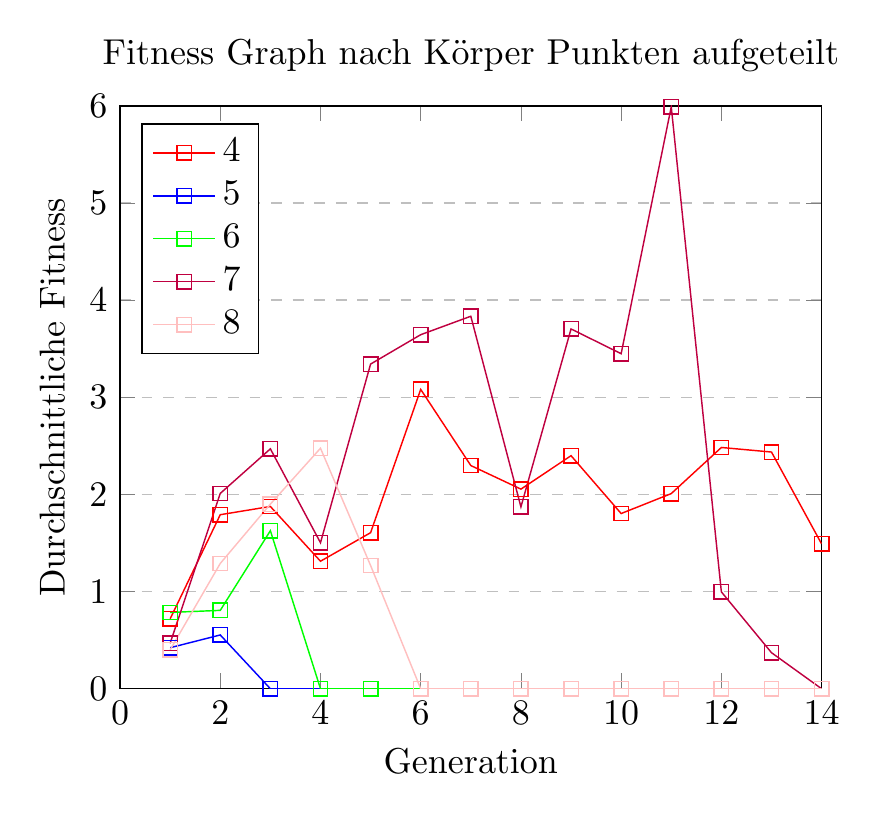
\begin{tikzpicture}[scale=1.3]
\begin{axis}[
    title={Fitness Graph nach Körper Punkten aufgeteilt},
    xlabel={Generation},
    ylabel={Durchschnittliche Fitness},
    xmin=0, xmax=14,
    ymin=0, ymax=6,
    xtick={0,2,4,6,8,10,12,14},
    ytick={0,1,2,3,4,5,6},
    legend pos=north west,
    ymajorgrids=true,
    grid style=dashed,
]

\addplot[
    color=red,
    mark=square,
    ]
    coordinates {
		(1,0.7197311288090767)(2,1.7917008390932372)(3,1.8763654203641982)(4,1.3127839017887504)(5,1.606485315324629)(6,3.081845732380266)(7,2.297797014315923)(8,2.055005581999147)(9,2.3994162926548404)(10,1.8036576432900295)(11,2.009064516425133)(12,2.4837885438165532)(13,2.436803859690654)(14,1.4910241046299537)
    };
    \addlegendentry{4}


\addplot[
    color=blue,
    mark=square,
    ]
    coordinates {
	(1,0.42241279780864716)(2,0.5535280124137276)(3,0)(4,0)(5,0)(6,0)(7,0)(8,0)(9,0)(10,0)(11,0)(12,0)(13,0)(14,0)
    };
    \addlegendentry{5}


\addplot[
    color=green,
    mark=square,
    ]
    coordinates {
	(1,0.7854441017622039)(2,0.8068950995802879)(3,1.6271000623703002)(4,0)(5,0)(6,0)(7,0)(8,0)(9,0)(10,0)(11,0)(12,0)(13,0)(14,0)
    };
    \addlegendentry{6}

\addplot[
    color=purple,
    mark=square,
    ]
    coordinates {
		(1,0.4685424281464469)(2,2.0108517235517502)(3,2.4697639744947937)(4,1.503244884001712)(5,3.3424592366328043)(6,3.644894652227138)(7,3.8348696411420136)(8,1.871792603770028)(9,3.70393052816391)(10,3.4490561534961066)(11,5.99130117893219)(12,0.9973328045823358)(13,0.37121231853961945)(14,0)
	};
    \addlegendentry{7}

\addplot[
    color=pink,
    mark=square,
    ]
    coordinates {
		(1,0.4001652509683654)(2,1.2898510225117206)(3,1.9010943668809803)(4,2.4758530855178833)(5,1.268694241841634)(6,0)(7,0)(8,0)(9,0)(10,0)(11,0)(12,0)(13,0)(14,0)
    };
    \addlegendentry{8}

\end{axis}
\end{tikzpicture}

    \caption{Durchschnittliches Individuum pro Anzahl Körper Punkte}
    \label{fig:graphBp}
  \end{figure}
